\chapter{Методи формалізації голосової інформації в системах диспетчерського контролю за рухом автотранспорту} \label{chapt3}

\section{Класифікація реакцій в системах диспетчерського контролю за рухом автотранспорту} \label{sect3_1}

Для створення класифікації реакцій в системах диспетчерського контролю за рухом автотранспорту було зібрано статистичні дані (зауваження та коментарі) щодо процесу доставки різних вантажів автомобільним транспортом у провідних логістичних компаніях. Систематизація та обробка зібраних оригінальних коментарів до статусу доставки, що використовуються в різних компаніях (табл. \ref{tbl:original_comments}), дали змогу створити відповідну до представленої на рис. \ref{img:voice_interaction_schema} моделі класифікацію голосових команд для субʼєктів дистрибуції «склад – дорога – точка доставки», яку подано нижче.

Для «складу» наявні такі головні коментарі:
\begin{itemize}
	\item проблеми з вантажем:
	\begin{itemize}
		\item відсутня частина товару на складі;
		\item забруднена продукція (пил, бруд, стійкий сторонній запах);
		\item частина товару пошкоджена;
		\item відсутня накладна;
		\item неправильно розраховано тоннаж та/або обʼєм продукції (товар не вміщується в авто);
	\end{itemize}
	\item проблеми з машиною:
	\begin{itemize}
		\item несправність ТЗ;
		\item машина не заводиться;
	\end{itemize}
	\item проблеми з виїздом:
	\begin{itemize}
		\item запізнення прибуття на склад;
		\item затримка завантаження товару на складі при вчасній подачі автомобіля;
	\end{itemize}
	\item інші команди:
	\begin{itemize}
		\item набрати диспетчера;
		\item показати маршрутний лист;
		\item показати мапу маршруту;
		\item виїзд зі складу.
	\end{itemize}
\end{itemize}

Для «дороги» наявні такі головні коментарі:
\begin{itemize}
	\item неможливо досягти точки:
	\begin{itemize}
		\item заблокований вʼїзд/виїзд автомобіля доставки;
		\item немає підʼїзду до будинку (будівельні, дорожні роботи, припаркований транспорт тощо), обʼїхати неможливо;
		\item неправильна адреса або недостатньо інформації для доставки замовлення;
		\item не знайшли адресу;
		\item не було місця для парковки;
		\item авто не змогло під`їхати через габарити;
	\end{itemize}
	\item складнощі з досягненням точки:
	\begin{itemize}
		\item неправильне присвоєння сектору/координат;
		\item похибка при складанні маршруту (адреса точки доставки випадає з логіки загального маршруту);
		\item підʼїзд до будинку з іншої вулиці;
	\end{itemize}
	\item затримки в русі, відхилення від маршруту, можливо, необхідний перерахунок маршруту:
	\begin{itemize}
		\item транспортний затор на маршруті;
		\item будівельні, дорожні роботи, перекриті дороги;
		\item помилка карти - маршрут прокладено по неіснуючій дорозі;
	\end{itemize}
	\item неможливо продовжувати маршрут:
	\begin{itemize}
		\item транспортний засіб потрапив у ДТП;
		\item поломка ТЗ на маршруті;
		\item складні погодні умови (автотранспорт фізично не може доїхати до місця доставки);
	\end{itemize}
	\item інші команди:
	\begin{itemize}
		\item набрати диспетчера;
		\item набрати клієнта;
		\item показати маршрутний лист;
		\item показати мапу маршруту;
		\item показати інформацію про точку;
		\item прибув у точку.
	\end{itemize}
\end{itemize}

Для «точки доставки» наявні такі головні коментарі:
\begin{itemize}
	\item відсутність клієнта:
	\begin{itemize}
		\item клієнт забув про доставку;
		\item особисті причини (клієнт не зміг бути вчасно);
		\item клієнта немає на місці, звʼязок з ним відсутній (некоректний номер телефону для звʼязку, недодзвін);
		\item невчасне (запізнення/випередження) прибуття на точку доставки, клієнт не має змоги прийняти товар;
	\end{itemize}
	\item немає можливості виконати доставку:
	\begin{itemize}
		\item не працює ліфт, клієнт проживає вище Х поверху;
		\item закрито доступ до приміщення клієнта;
		\item у клієнта відсутні необхідні документи, матеріали чи товар для відвантаження;
	\end{itemize}
	\item відмова клієнта прийняти товар:
	\begin{itemize}
		\item відмова на місці;
		\item немає грошей;
		\item пошкоджений або відсутній товар:
		\begin{itemize}
			\item товар не завантажено;
			\item товар забруднений;
			\item товар недоукомплектовано;
			\item товар не працює (внутрішня поломка);
			\item товар пошкоджено зовні;
		\end{itemize}
	\end{itemize}
	\item помилка в замовленні:
	\begin{itemize}
		\item не робили замовлення взагалі;
		\item замовляли на інший день;
		\item замовляли на іншу адресу;
		\item замовляли на інший час;
		\item замовляли інший товар;
	\end{itemize}
	\item часткове виконання замовлення:
	\begin{itemize}
		\item задвоєне замовлення, половина товару повертається;
		\item у документах зазначено товар, який клієнт не замовляв;
	\end{itemize}
	\item інші команди:
	\begin{itemize}
		\item набрати диспетчера;
		\item набрати клієнта;
		\item показати маршрутний лист;
		\item показати мапу маршруту;
		\item показати інформацію про точку;
		\item почав виконання наступної точки;
		\item точка успішно виконана.
	\end{itemize}
\end{itemize}

\section{Модель голосової взаємодії водія в системах диспетчерського контролю за рухом автотранспорту} \label{sect3_2}

\subsection{Побудова орієнтованого графу сценаріїв голосової взаємодії}

Як зазначалося в попередньому розділі, дерево сценаріїв може бути застосоване для голосової взаємодії субʼєктів дистрибуції «склад – дорога – точка доставки» відповідно до моделі, що наведена на рис. \ref{img:voice_interaction_schema}. Найпростіше дерево сценаріїв для моделі голосової взаємодії водія в системах диспетчерського контролю за рухом автотранспорту можна представити в такий спосіб (рис. \ref{img:01_simplest_positive_scenario}).

\begin{figure}
	\centering
	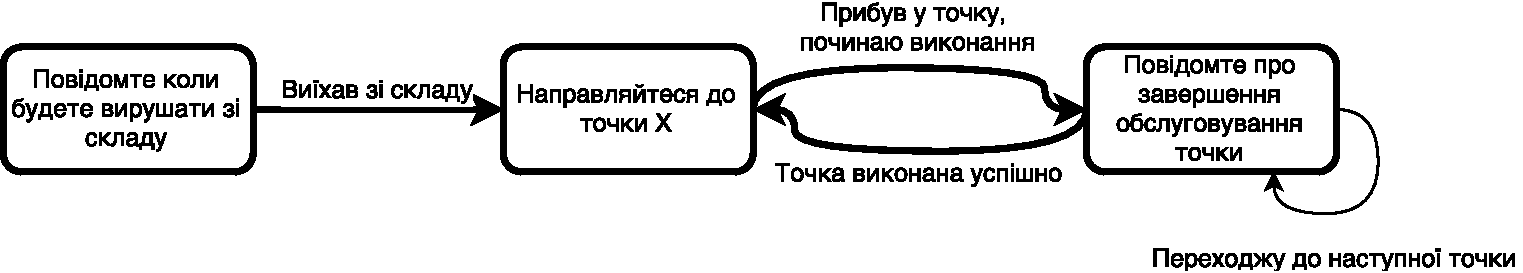
\includegraphics [width=1\linewidth] {01_simplest_positive_scenario}
	\caption{Найпростіше дерево сценаріїв}
	\label{img:01_simplest_positive_scenario}
\end{figure}

Таке саме найпростіше дерево сценаріїв для моделі голосової взаємодії водія в системах диспетчерського контролю за рухом автотранспорту тільки з вертикальним розподілом наведено на рис. \ref{img:02_simplest_positive_scenario_vertical}.

\begin{figure}
	\centering
	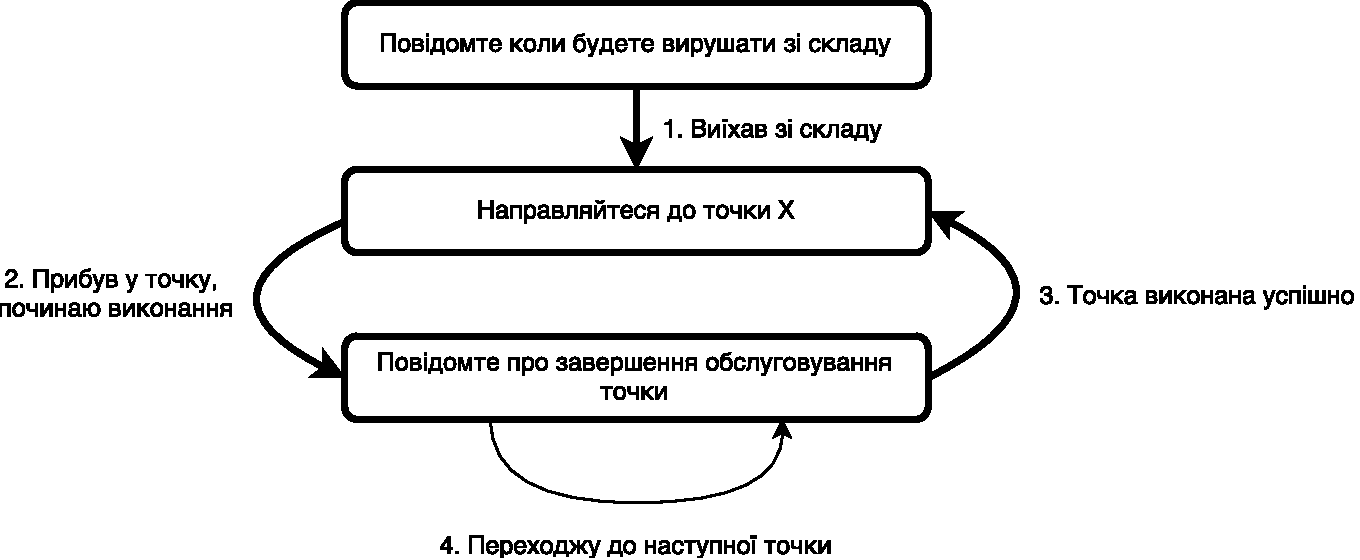
\includegraphics [width=1\linewidth] {02_simplest_positive_scenario_vertical}
	\caption{Вертикальний розподіл найпростішого дерева сценаріїв}
	\label{img:02_simplest_positive_scenario_vertical}
\end{figure}

Найпростіше дерево сценаріїв (рис. \ref{img:01_simplest_positive_scenario}, \ref{img:02_simplest_positive_scenario_vertical}) показує всі доступні варіанти (послідовність подій) в моделі голосової взаємодії водія в системах диспетчерського контролю за рухом автотранспорту. Кожна така послідовність (або ланцюжок) подій повинна представлятися окремим сценарієм.

Для випадку позитивного підтвердження обслуговування або виконання відповідної точки в моделі голосової взаємодії водія в системах диспетчерського контролю за рухом автотранспорту побудовано позитивне дерево сценаріїв (рис. \ref{img:03_positive_scenario_with_conformation}).

\begin{figure}
	\centering
	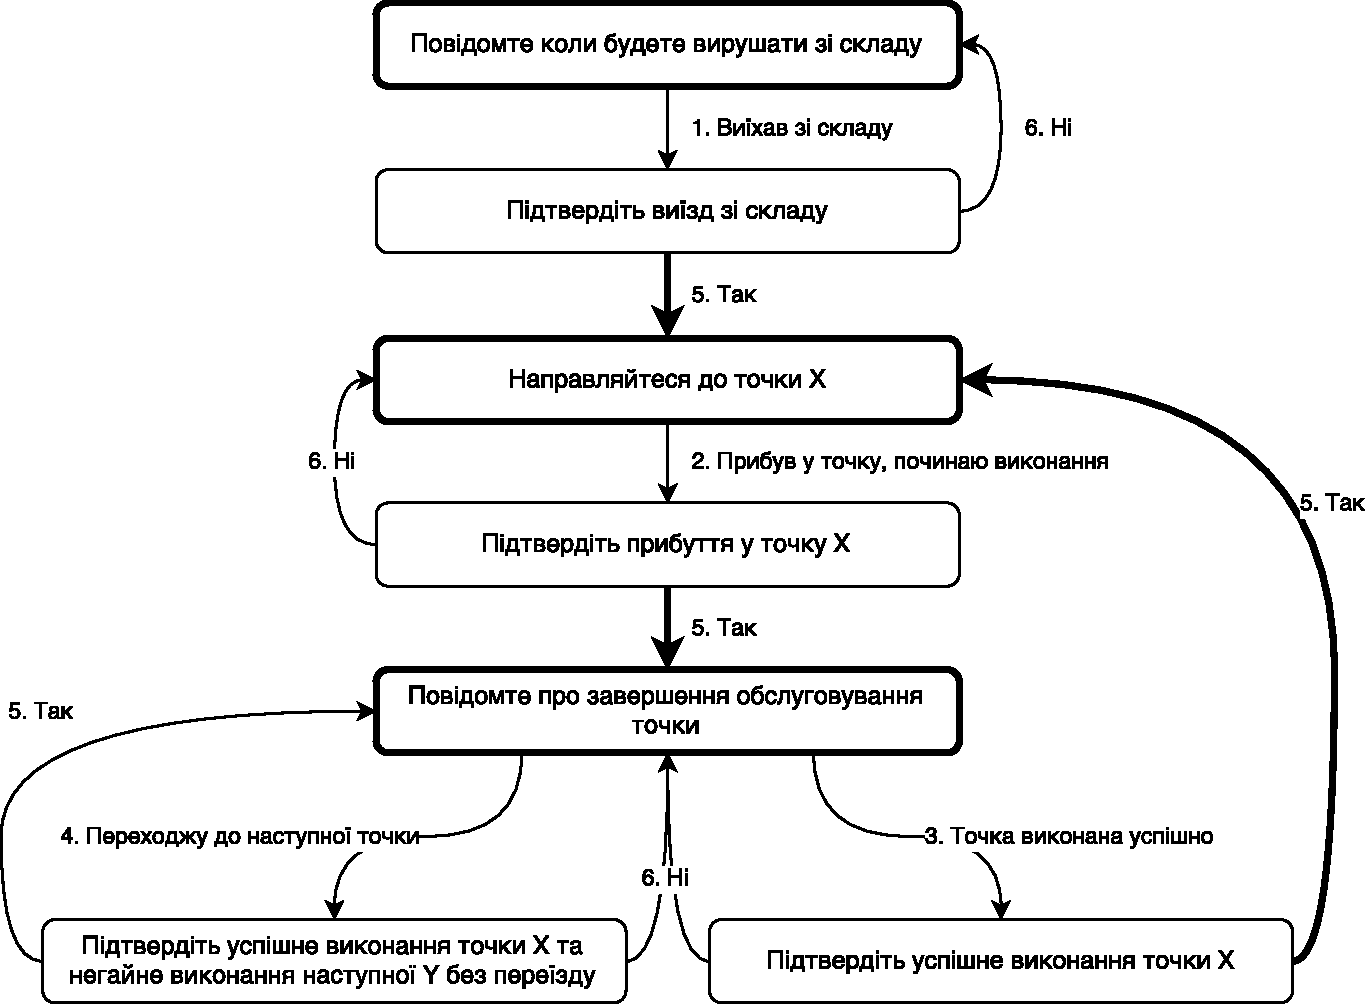
\includegraphics [width=1\linewidth] {03_positive_scenario_with_conformation}
	\caption{Позитивне дерево сценаріїв з підтвердженням}
	\label{img:03_positive_scenario_with_conformation}
\end{figure}

Наведене позитивне дерево сценаріїв з підтвердженням обслуговування або виконання відповідної точки (рис. \ref{img:03_positive_scenario_with_conformation}) є більш складним порівняно з найпростішим деревом сценаріїв (рис. \ref{img:01_simplest_positive_scenario}, \ref{img:02_simplest_positive_scenario_vertical}).  Це ключова відмінність цього дерева від попереднього, де враховано можливість відміни команди, помилково розпізнаної системою, або помилкової команди водія. Позитивне дерево сценаріїв є достатнім для ідеального світу, де все відбувається за планом. Як бачимо, для даного випадку обслуговування або виконання відповідної точки відбувається без позапланових ситуацій на відміну від дерева сценаріїв з негативними інцидентами, перший варіант якого наведено на рис. \ref{img:04_first_negative_scenario_with_conformation}.

На рис. \ref{img:04_first_negative_scenario_with_conformation} зʼявляється додатковий блок, повʼязаний з підтвердженням того, що точку Х не вдалося виконати, тобто дерево сценаріїв враховує можливі негативні інциденти в моделі голосової взаємодії водія в системах диспетчерського контролю за рухом автотранспорту.

\begin{figure}
	\centering
	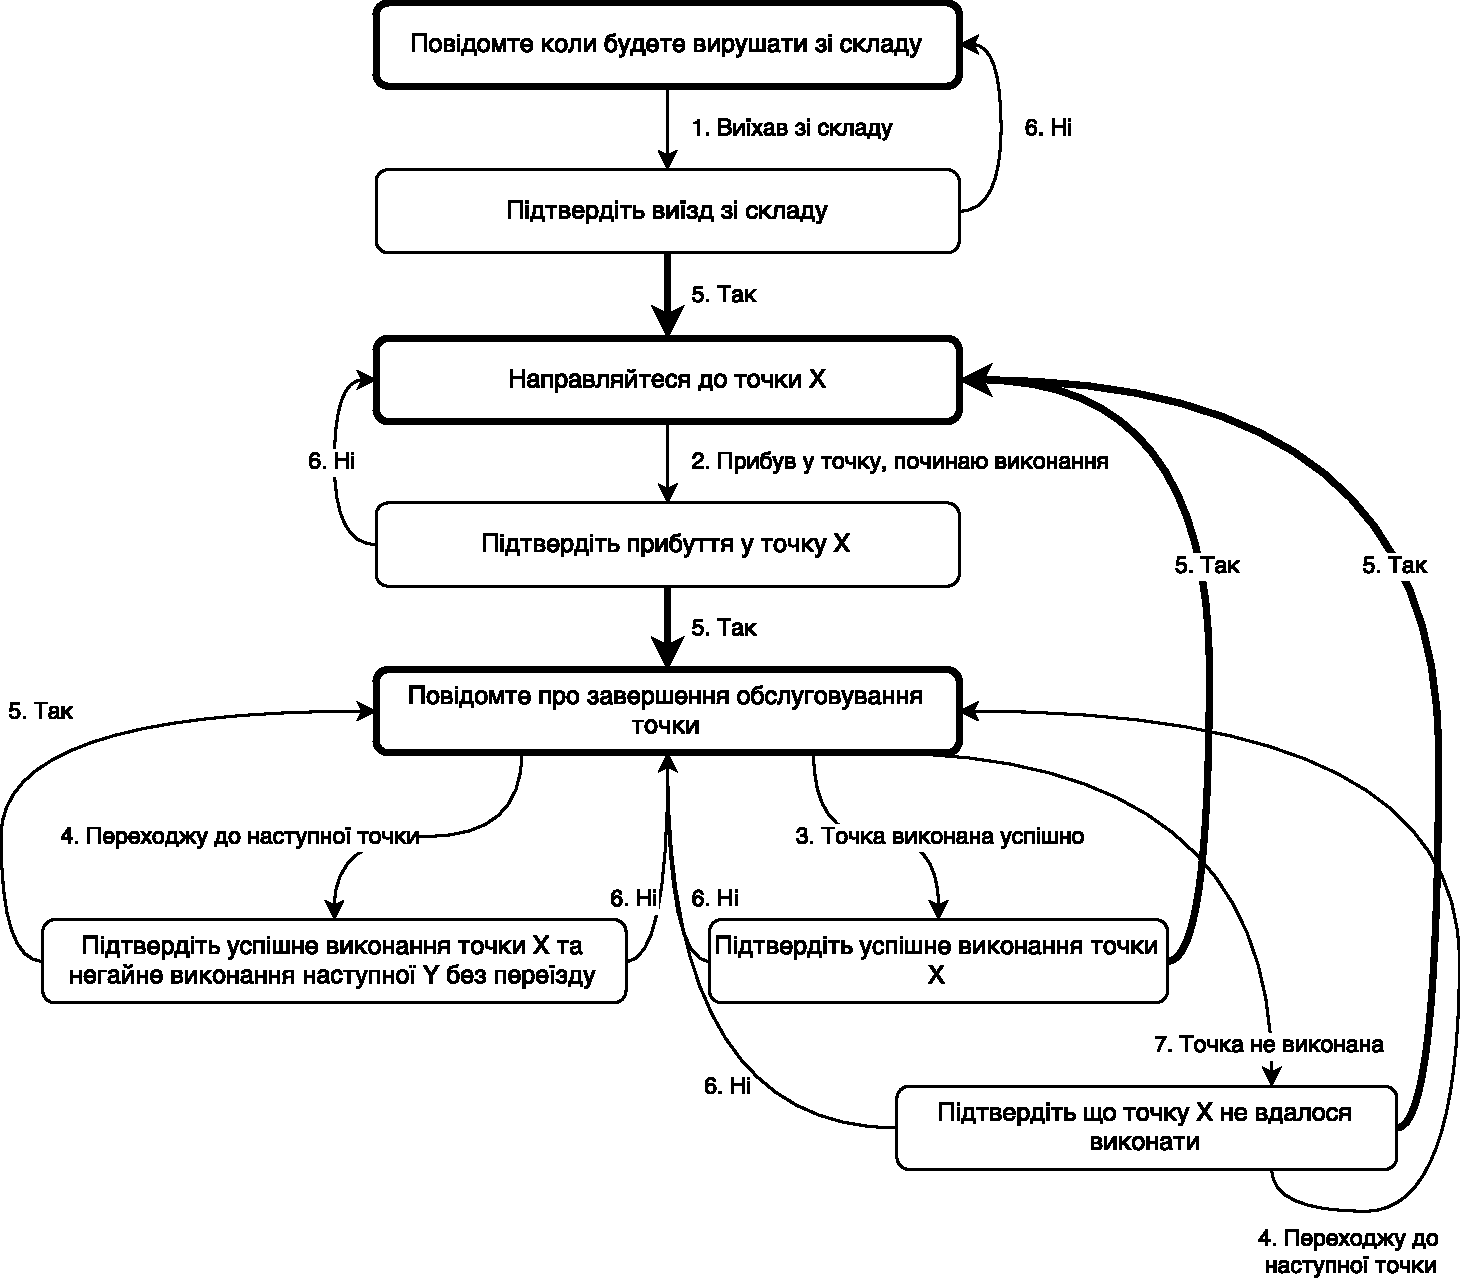
\includegraphics [width=1\linewidth] {04_first_negative_scenario_with_conformation}
	\caption{Перший варіант дерева сценаріїв з негативними інцидентами}
	\label{img:04_first_negative_scenario_with_conformation}
\end{figure}

Спрощений варіант дерева сценаріїв у моделі голосової взаємодії водія в системах диспетчерського контролю за рухом автотранспорту з негативними інцидентами наведено на рис. \ref{img:05_simple_negative_scenario_with_conformation}. У цьому варіанті блок з підтвердженням успішного виконання точки Х, з негайним виконанням наступної точки Y без переїзду трансформується в блок, повʼязаний з підтвердженням того, що точку Х не вдалося виконати, і стає, по суті, спрощеним варіантом дерева сценаріїв з негативними інцидентами, що наведений на рис. \ref{img:04_first_negative_scenario_with_conformation}.

\begin{figure}
	\centering
	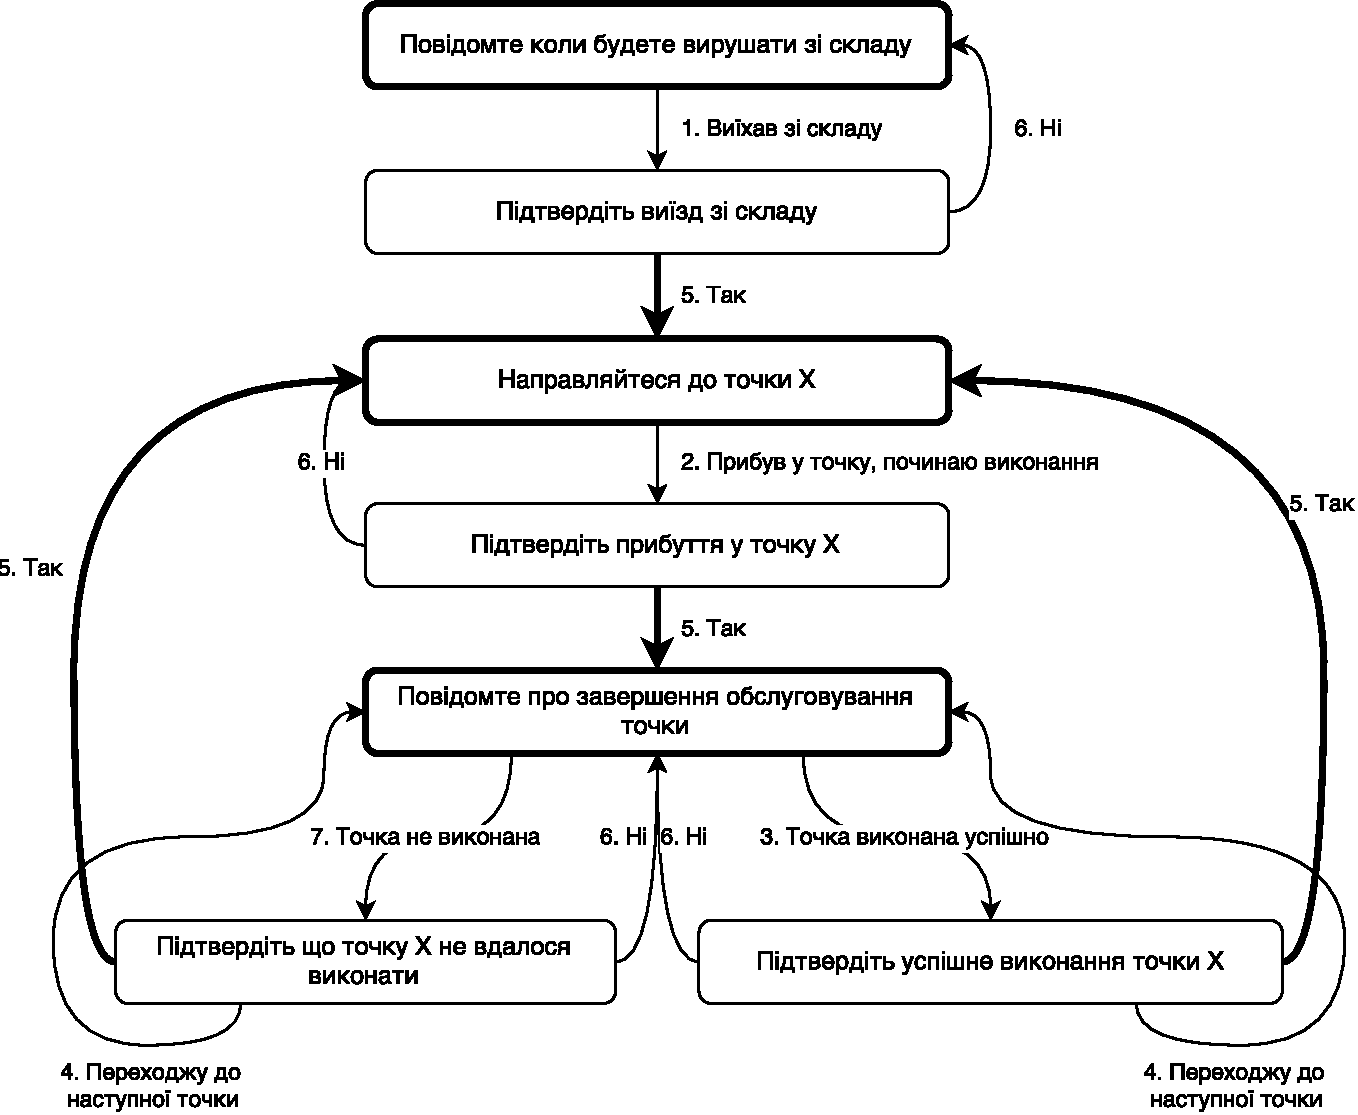
\includegraphics [width=1\linewidth] {05_simple_negative_scenario_with_conformation}
	\caption{Спрощений варіант дерева сценаріїв з негативними інцидентами}
	\label{img:05_simple_negative_scenario_with_conformation}
\end{figure}

Також у моделі голосової взаємодії водія в системах диспетчерського контролю за рухом автотранспорту може бути запропонований один з варіантів дерева сценаріїв з негативними інцидентами та відміною виконання ("відбоєм") (рис. \ref{img:06_simple_negative_scenario_with_rollback}). Для наведеного випадку в дереві сценаріїв зʼявляється блок, повʼязаний з підтвердженням неприбуття в точку Х. Тобто, в дереві сценаріїв зʼявляється звʼязок з відміною виконання та обслуговування точки Х при моделюванні голосової взаємодії водія в системах диспетчерського контролю за рухом автотранспорту. У "спрощеному" варіанті прибирається додаткове підтвердження для "переходжу до наступної точки". Щоб зберегти стійкість до помилок і простоту діалогу, замість підтвердження додаємо можливість відмінити цю останню дію.

\begin{figure}
	\centering
	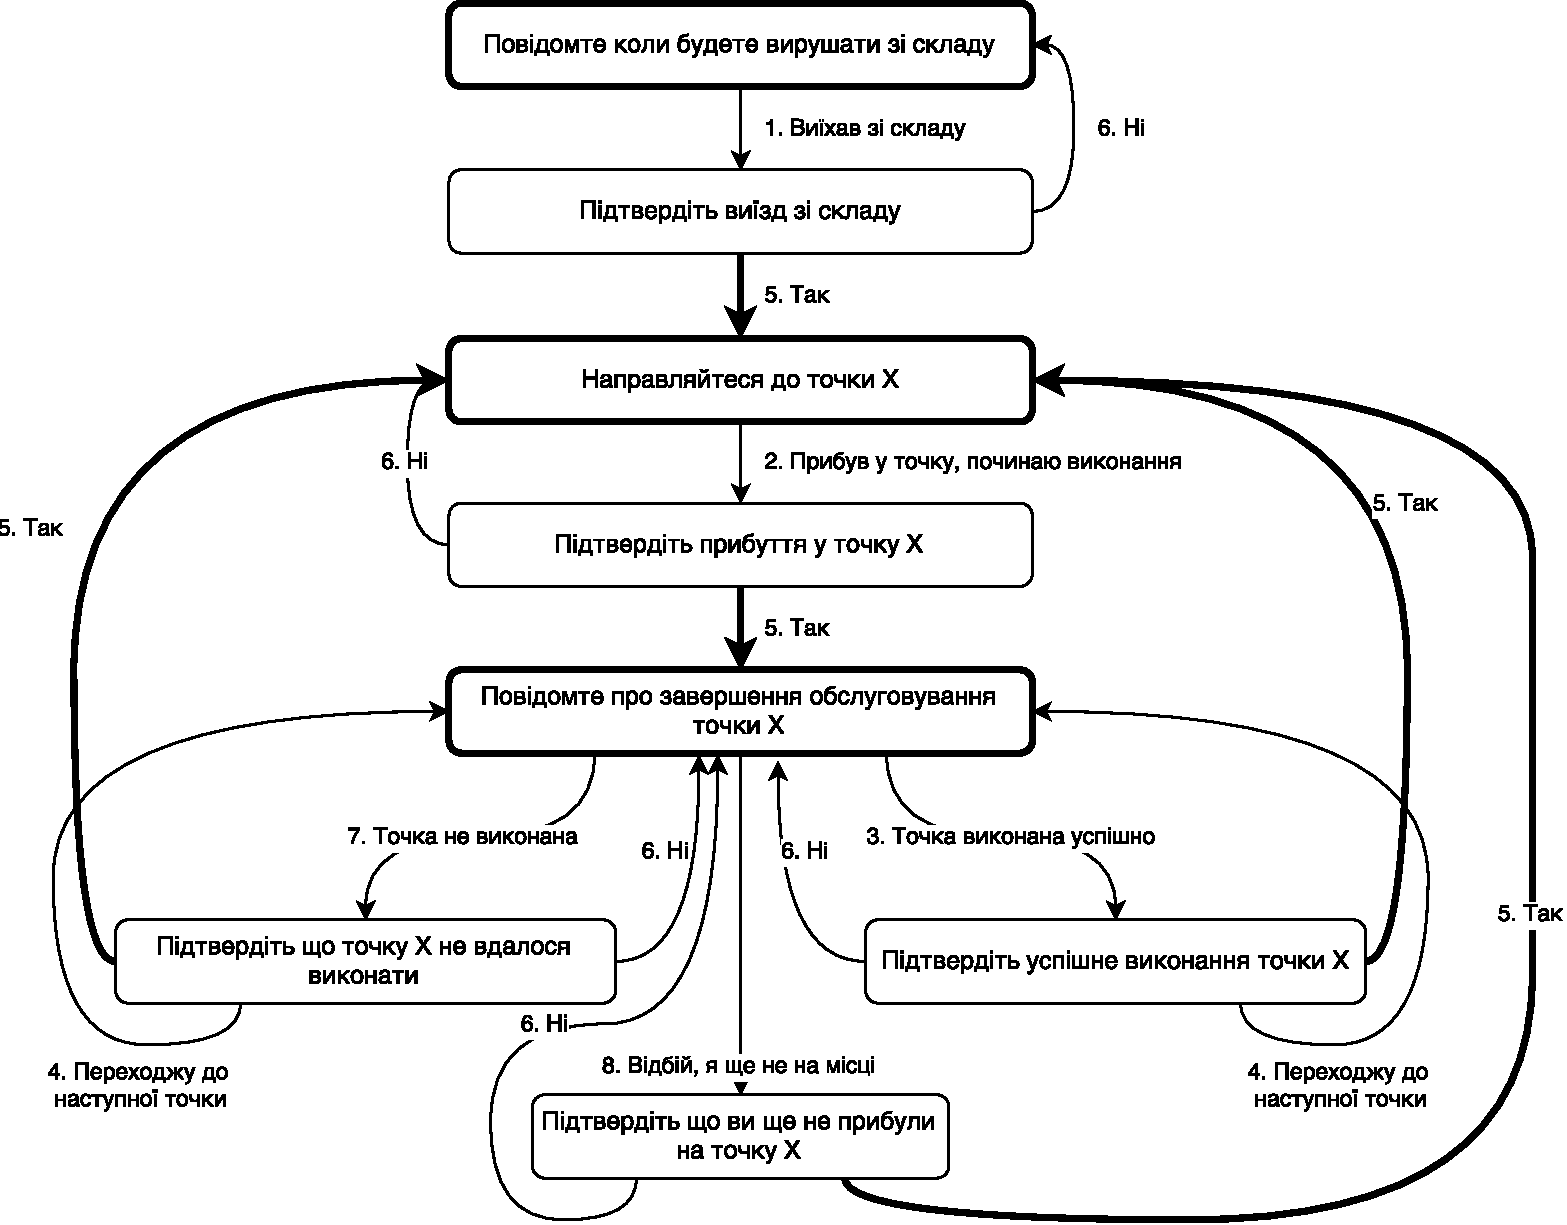
\includegraphics [width=1\linewidth] {06_simple_negative_scenario_with_rollback}
	\caption{Варіант дерева сценаріїв з негативними інцидентами та відбоєм}
	\label{img:06_simple_negative_scenario_with_rollback}
\end{figure}

Оскільки дерево стає занадто великим для зображення, для подальшої деталізації розібʼємо його на частини відповідно до трьох основних етапів. Частину дерева сценаріїв етапу «точка доставки» у вертикальному розподілі наведено на рис. \ref{img:07_simple_point_scenario}, у горизонтальному – на рис. \ref{img:07_simple_point_scenario_horizontal}.
Наведені фрагменти дерева сценаріїв етапу «точка доставки» у вертикальному (рис. \ref{img:07_simple_point_scenario}) та горизонтальному (рис. \ref{img:07_simple_point_scenario_horizontal}) розподілах містять виконання та обслуговування попередньої точки Y, поточної точки Х та наступної точки Z, що розташовані на відповідних дорогах.

\begin{figure}
	\centering
	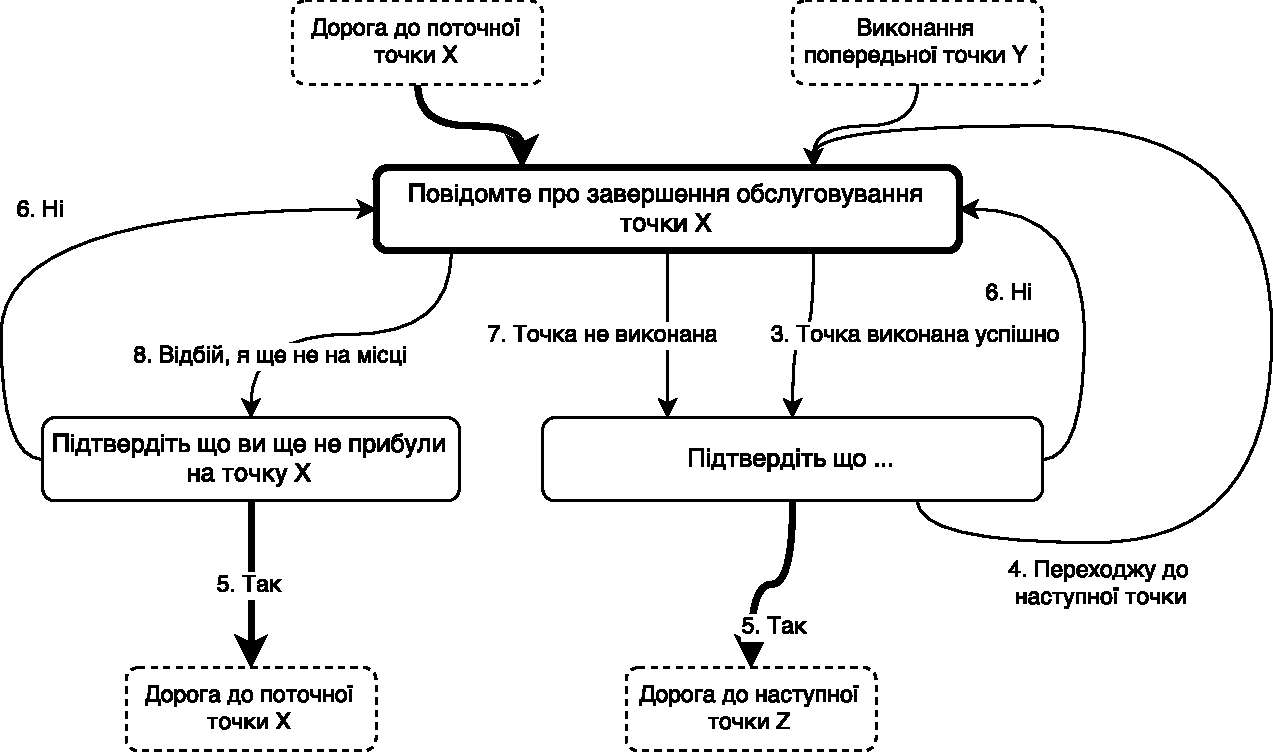
\includegraphics [width=1\linewidth] {07_simple_point_scenario}
	\caption{Частина дерева сценаріїв етапу <<точка доставки>>}
	\label{img:07_simple_point_scenario}
\end{figure}

\begin{figure}
	\centering
	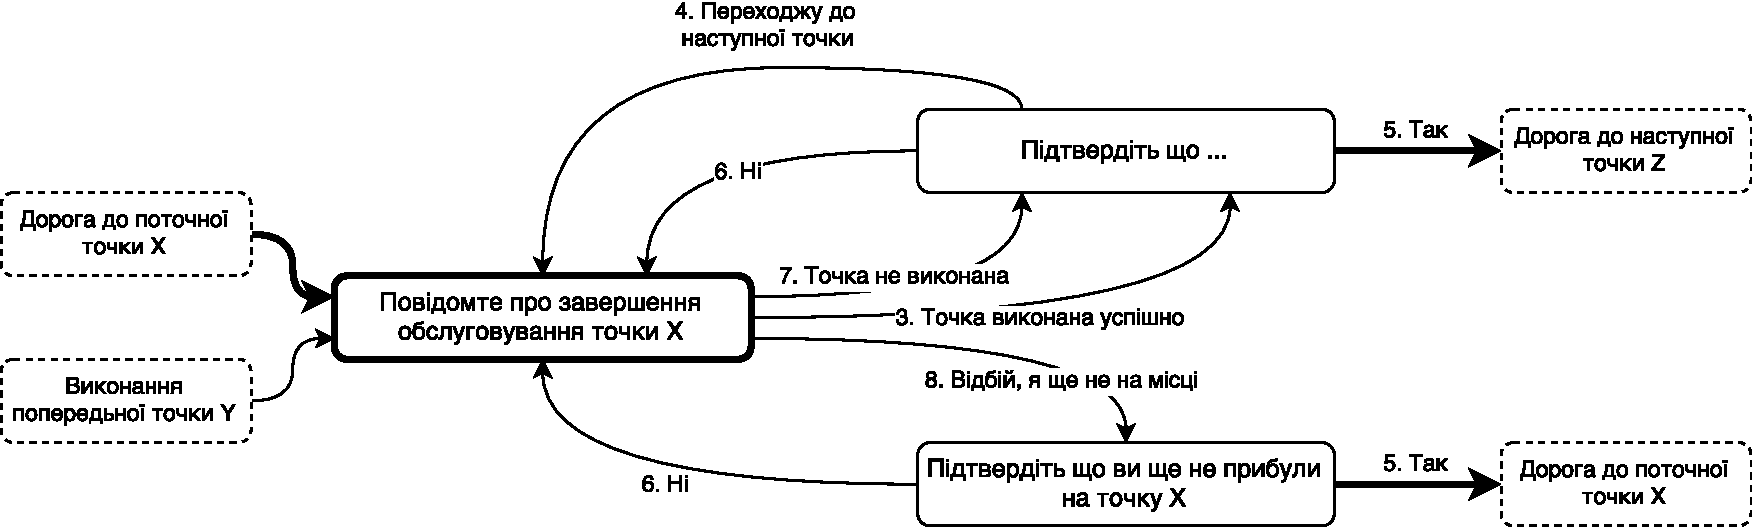
\includegraphics [width=1\linewidth] {07_simple_point_scenario_horizontal}
	\caption{Частина дерева сценаріїв етапу <<точка доставки>> в горизонтальному розподілі}
	\label{img:07_simple_point_scenario_horizontal}
\end{figure}

Як бачимо з рис. \ref{img:07_simple_point_scenario} та \ref{img:07_simple_point_scenario_horizontal}, горизонтальний розподіл є більш компактним.
На рис. \ref{img:08_complete_point_scenario} наведено одну з частин дерева сценаріїв етапу «точка доставки» з усіма негативними інцидентами при моделюванні голосової взаємодії водія в системах диспетчерського контролю за рухом автотранспорту.


\begin{figure}
	\centering
	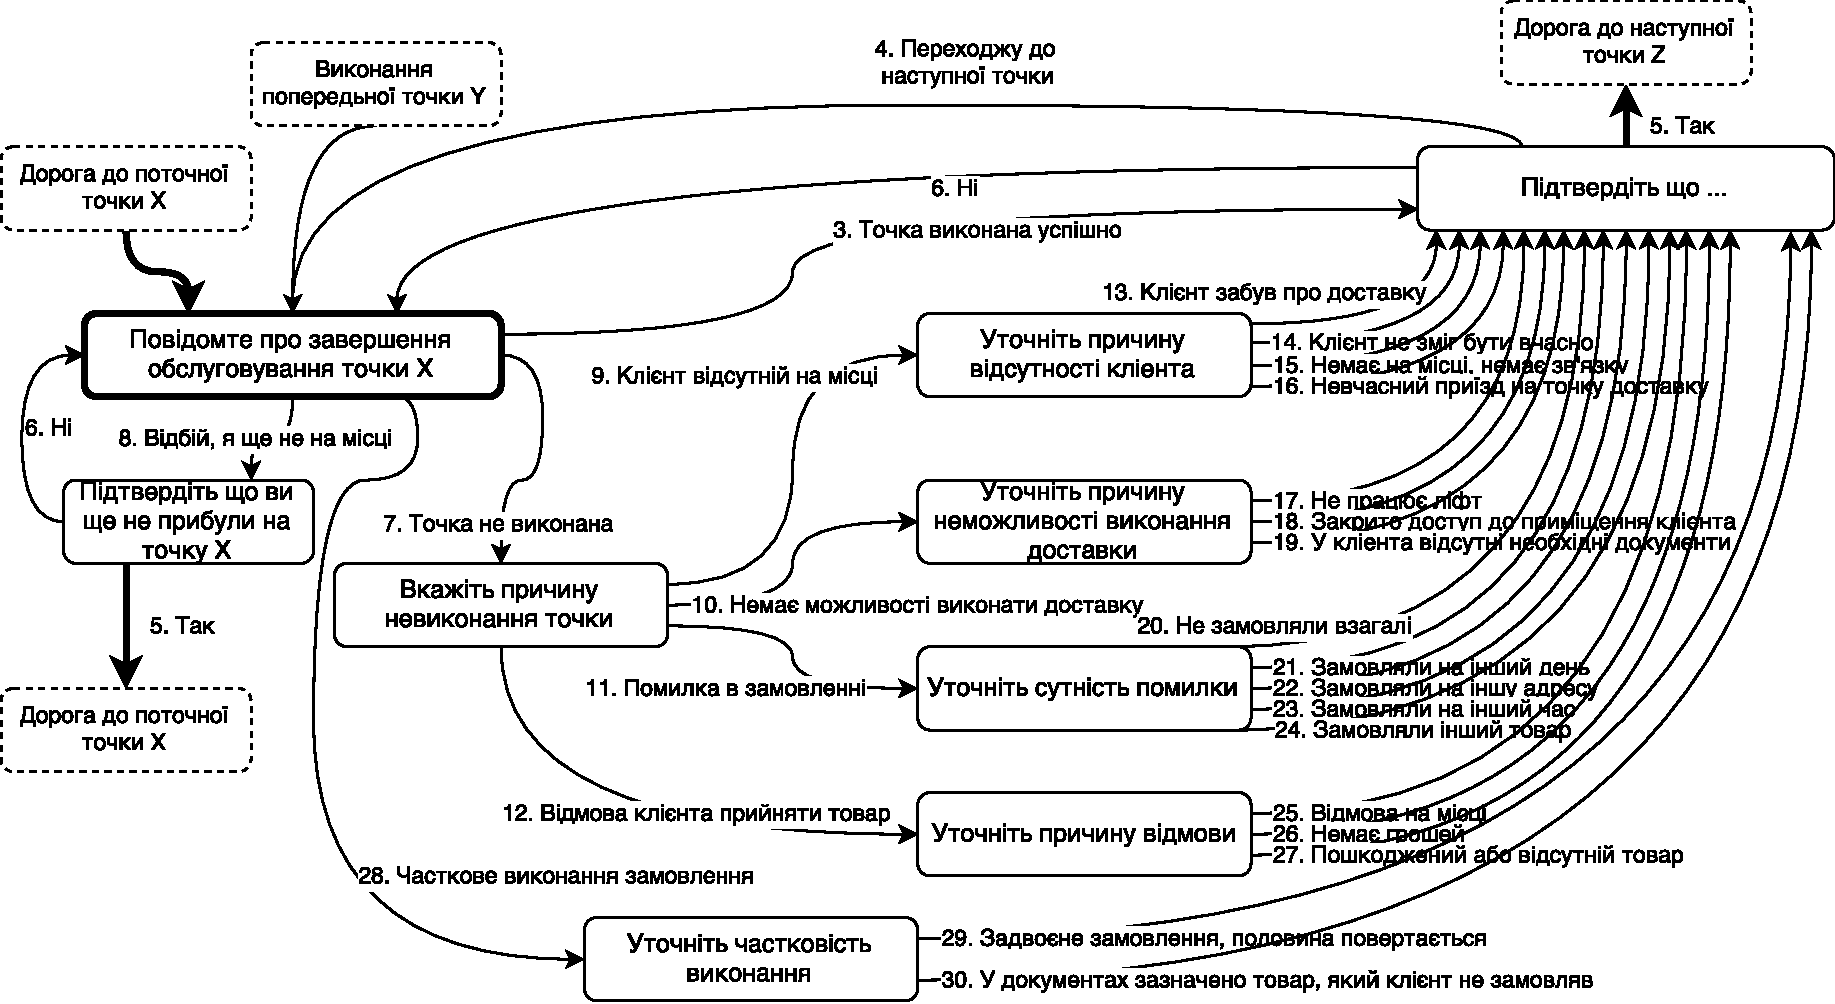
\includegraphics [width=1\linewidth] {08_complete_point_scenario}
	\caption{Частина дерева сценаріїв етапу <<точка доставки>> з усіма негативними інцидентами}
	\label{img:08_complete_point_scenario}
\end{figure}

Наведена частина дерева сценаріїв етапу «точка доставки» (рис. \ref{img:08_complete_point_scenario}) містить блок невиконання точки Х з розширеним уточненням причин та блок часткового виконання з характеристиками такого виконання.

На рис. \ref{img:08_complete_point_scenario_with_other} представлено частину дерева сценаріїв етапу «точка доставки» з усіма негативними інцидентами та врахуванням деяких інших непередбачених подій невиконання точки Х з більш розширеним уточненням причин порівняно з деревом сценаріїв, що представлено на рис. \ref{img:08_complete_point_scenario}, та частковим виконанням з більш розширеними характеристиками такого часткового виконання. Для зберігання відкритості досліджуваної системи на етапі моделювання не можуть бути враховані всі можливі варіанти розвитку подій, тому на рис. \ref{img:08_complete_point_scenario_with_other} наведено деякі непередбачувані події невиконання точки Х.

\begin{figure}
	\centering
	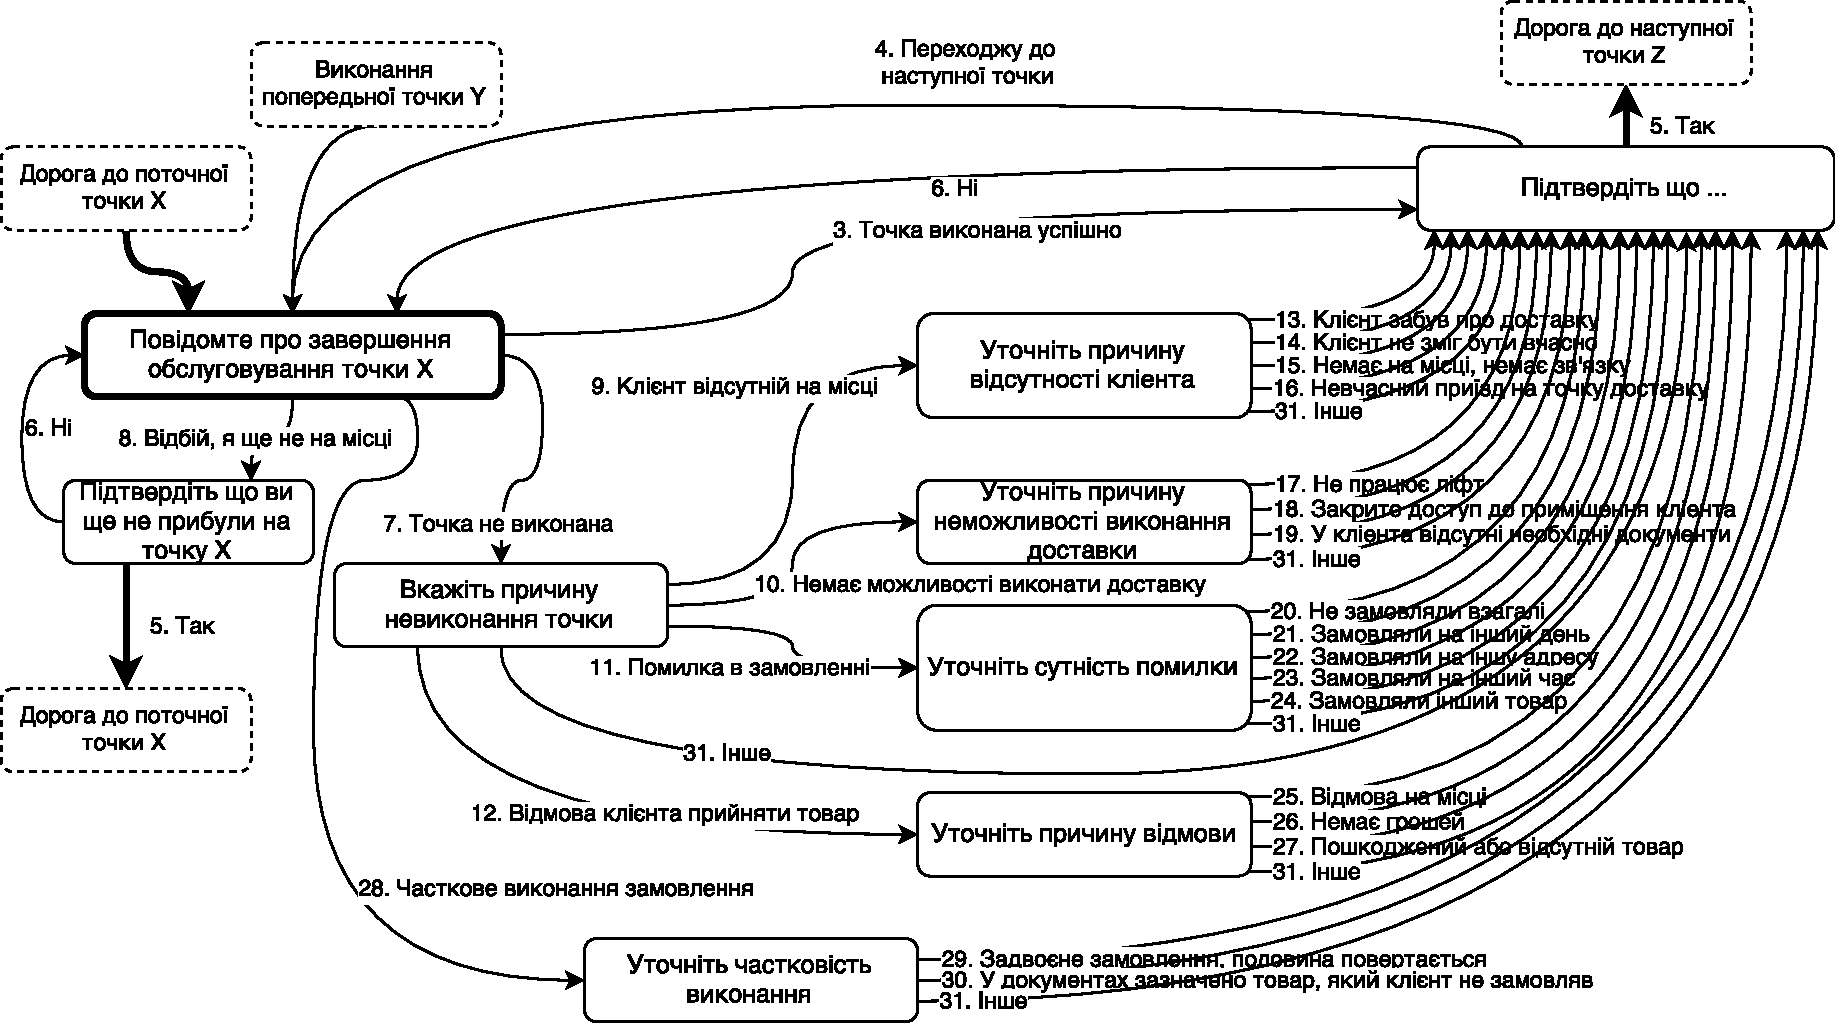
\includegraphics [width=1\linewidth] {08_complete_point_scenario_with_other}
	\caption{Частина дерева сценаріїв етапу <<точка доставки>> з усіма негативними інцидентами та урахуванням інших непередбачених подій}
	\label{img:08_complete_point_scenario_with_other}
\end{figure}

На рис. \ref{img:09_complete_point_scenario_with_rollback} представлено частину дерева сценаріїв етапу «точка доставки» з усіма негативними інцидентами та відбоєм із діалогового режиму. Можемо бачити, що для випадку відбою причин невиконання точки Х із діалогового режиму відбувається перехід до констатації обслуговування та успішного виконання точки Х при моделюванні голосової взаємодії водія в системах диспетчерського контролю за рухом автотранспорту.

\begin{figure} 
	\centering
	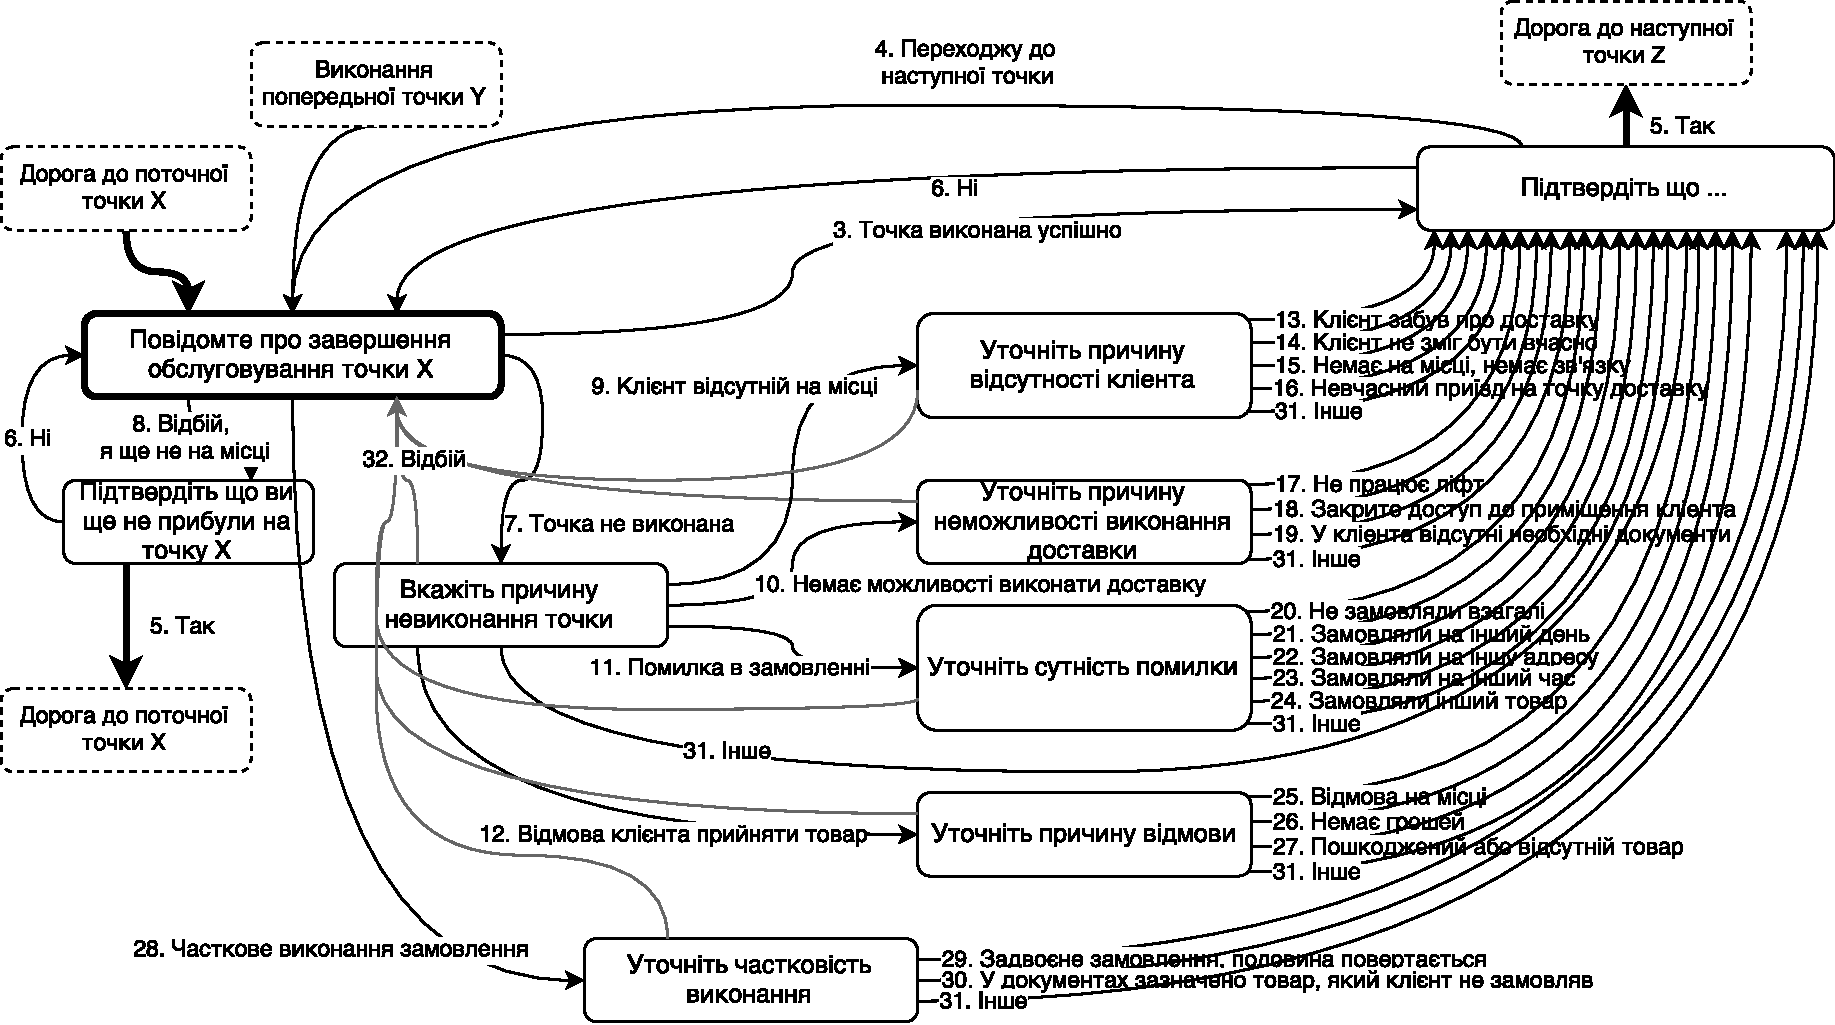
\includegraphics [width=1\linewidth] {09_complete_point_scenario_with_rollback}
	\caption{Частина дерева сценаріїв етапу "точка доставки" з усіма негативними інцидентами та відбоєм із діалогового режиму}
	\label{img:09_complete_point_scenario_with_rollback}
\end{figure}

Для випадку застосування додаткових функцій при моделюванні голосової взаємодії водія в системах диспетчерського контролю за рухом автотранспорту побудовано дерево сценаріїв етапу «точка доставки», частину якого наведено на рис. \ref{img:10_point_scenario_with_enchantment}.

\begin{figure}
	\centering
	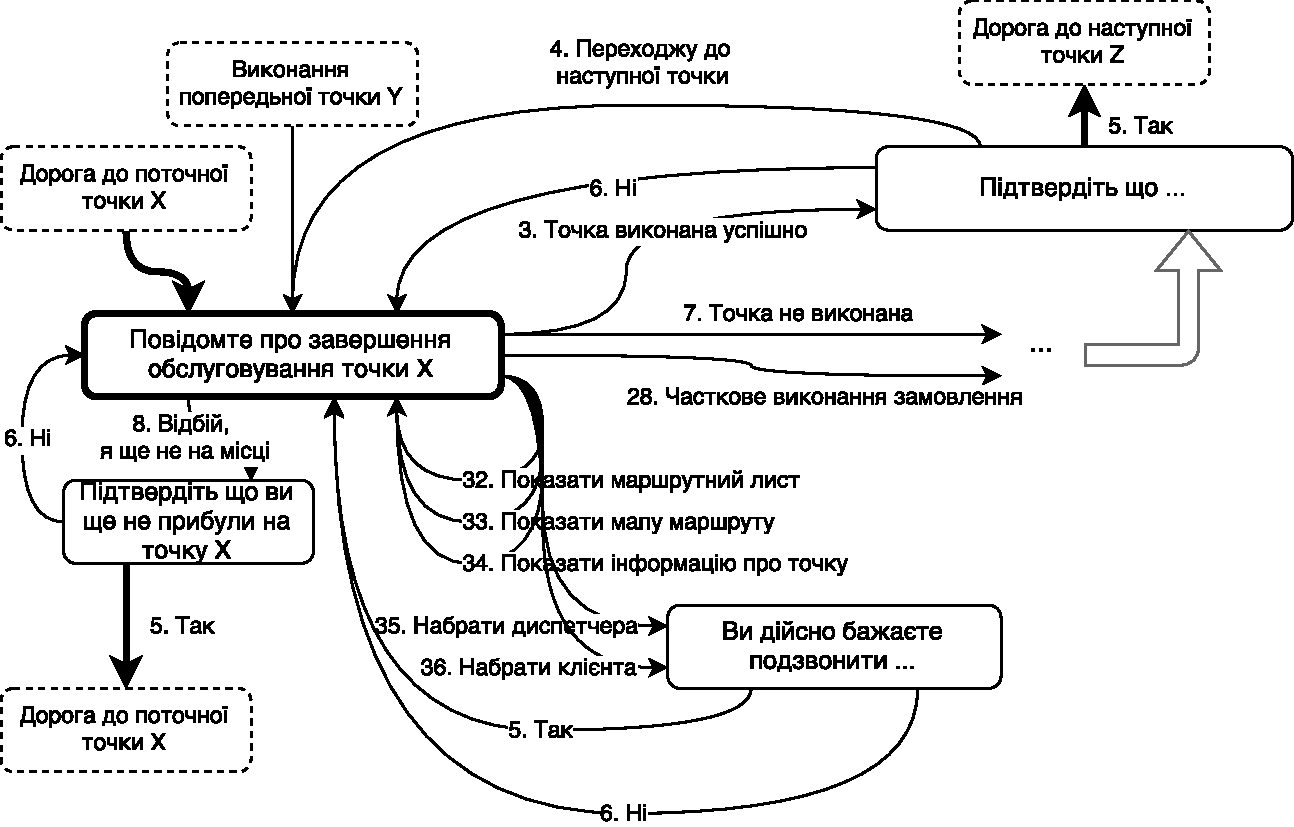
\includegraphics [width=1\linewidth] {10_point_scenario_with_enchantment}
	\caption{Частина дерева сценаріїв етапу <<точка доставки>> з додатковими функціями}
	\label{img:10_point_scenario_with_enchantment}
\end{figure}

У наведеній частині дерева сценаріїв етапу «точка доставки» (рис. \ref{img:10_point_scenario_with_enchantment}) присутні додаткові функції для водія при моделюванні його голосової взаємодії, повʼязані з інформаційними характеристиками маршруту до точки доставки Х, а також функції для набору диспетчера або клієнта.

На етапі «дорога» дерево сценаріїв для моделі голосової взаємодії водія в системах диспетчерського контролю за рухом автотранспорту має наступний вигляд (рис. \ref{img:11_complete_road_scenario}). У наведеній частині дерева сценаріїв етапу «дорога» враховано всі контексти з репрезентативної вибірки даних, які отримано у провідних логістичних компаніях України. При цьому, у випадку невиконання етапу «дорога» пропонуються причини затримки чи неможливості виконання маршруту з наступними інструкціями диспетчера, а у випадку, коли зʼявляється можливість виконання маршруту до точки доставки Х, існує відбій із діалогового режиму.

\begin{figure}
	\centering
	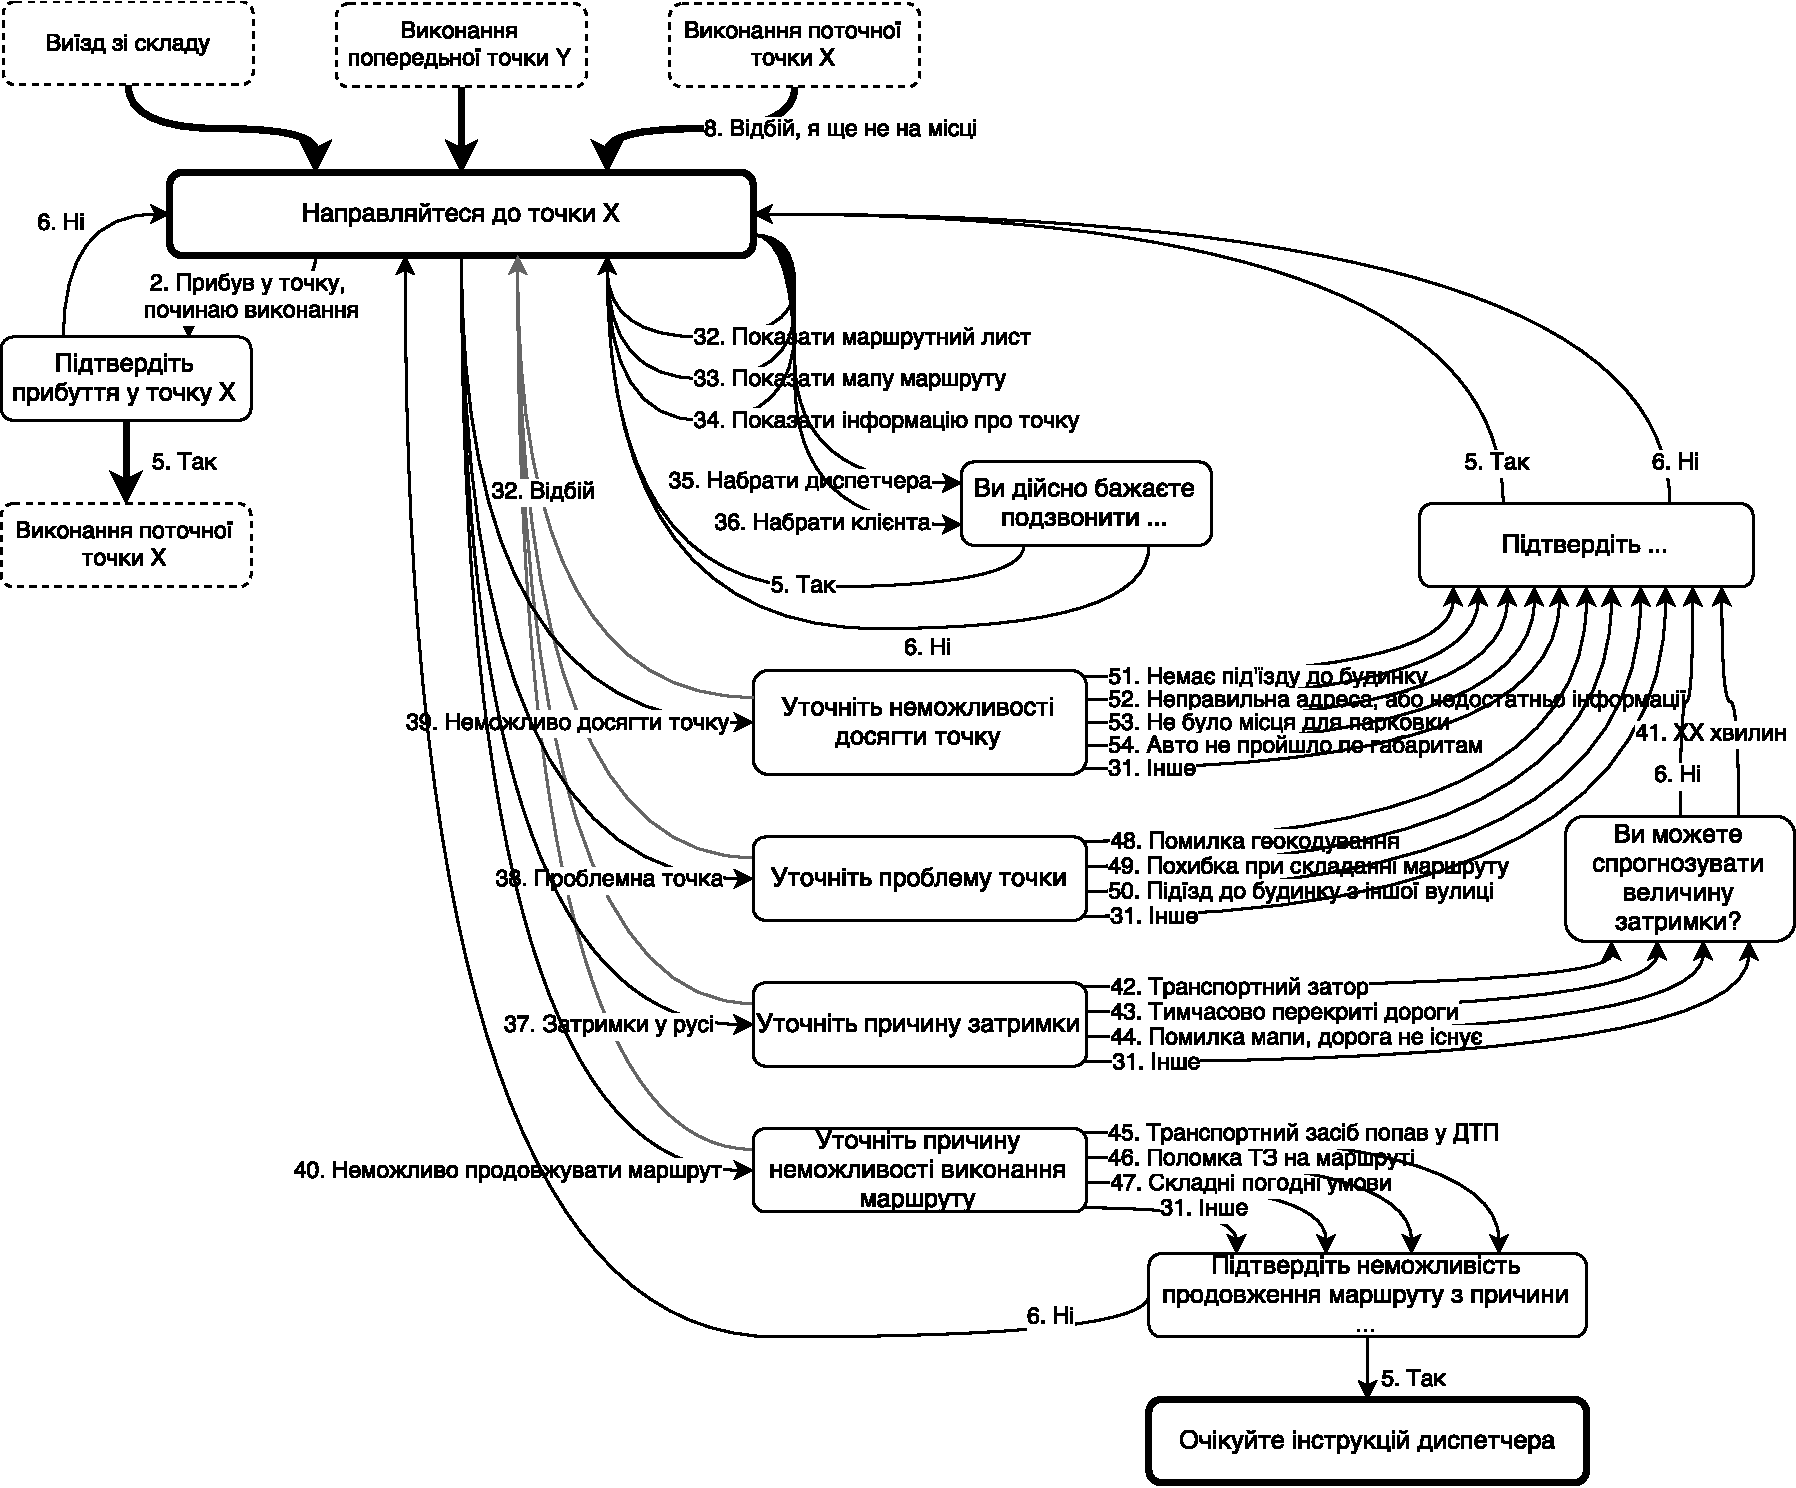
\includegraphics [width=.8\linewidth] {11_complete_road_scenario}
	\caption{Частина дерева сценаріїв етапу <<дорога>>}
	\label{img:11_complete_road_scenario}
\end{figure}

\begin{figure}
	\centering
	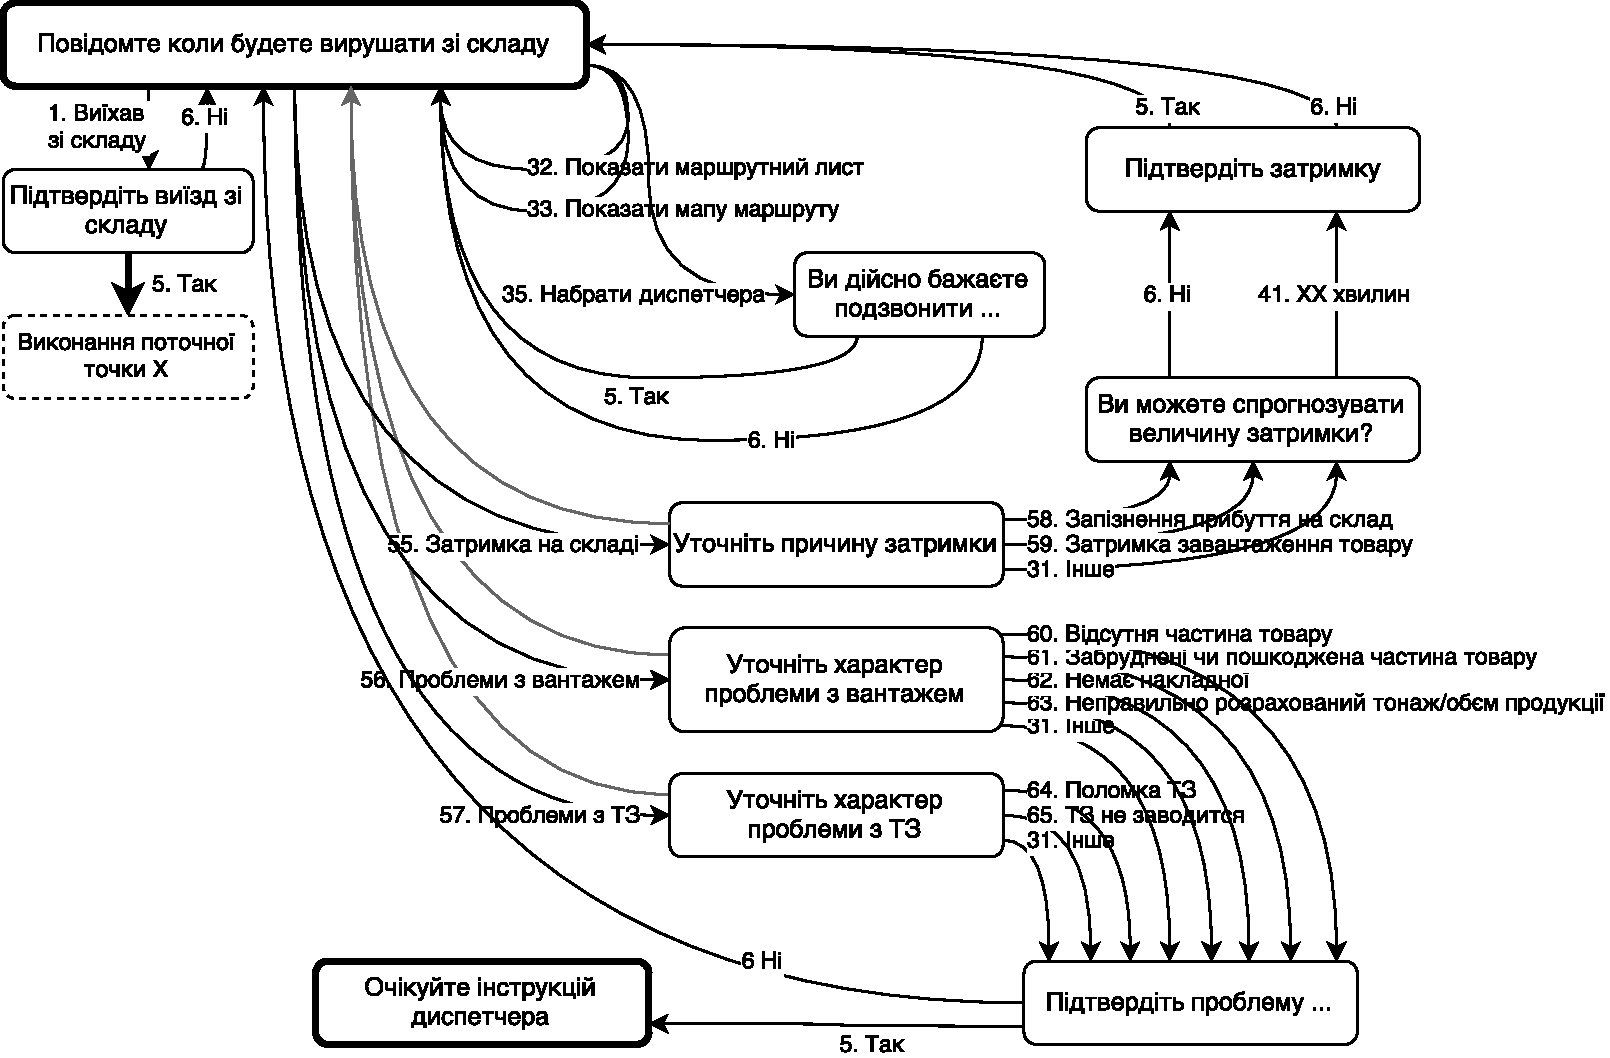
\includegraphics [width=.8\linewidth] {12_complete_depot_scenario}
	\caption{Частина дерева сценаріїв етапу <<склад>>}
	\label{img:12_complete_depot_scenario}
\end{figure}

Для виконання етапу «склад» субʼєктом дистрибуції – водієм при його голосовій взаємодії в системі диспетчерського контролю за рухом автотранспорту побудовано дерево сценаріїв етапу «склад», частину якого наведено на рис. \ref{img:12_complete_depot_scenario}.

У побудованому дереві сценаріїв етапу «склад» враховано причини затримки чи невиїзду зі складу з можливістю отримати подальші інструкції диспетчера для вирішення проблеми.

Повне дерево сценаріїв усіх етапів дистрибуції «склад – дорога – точка доставки» в моделі голосової взаємодії водія в системі диспетчерського контролю за рухом автотранспорту представлено на рис. \ref{img:13_complete_scenario_graph}.

\begin{figure}
	\centering
	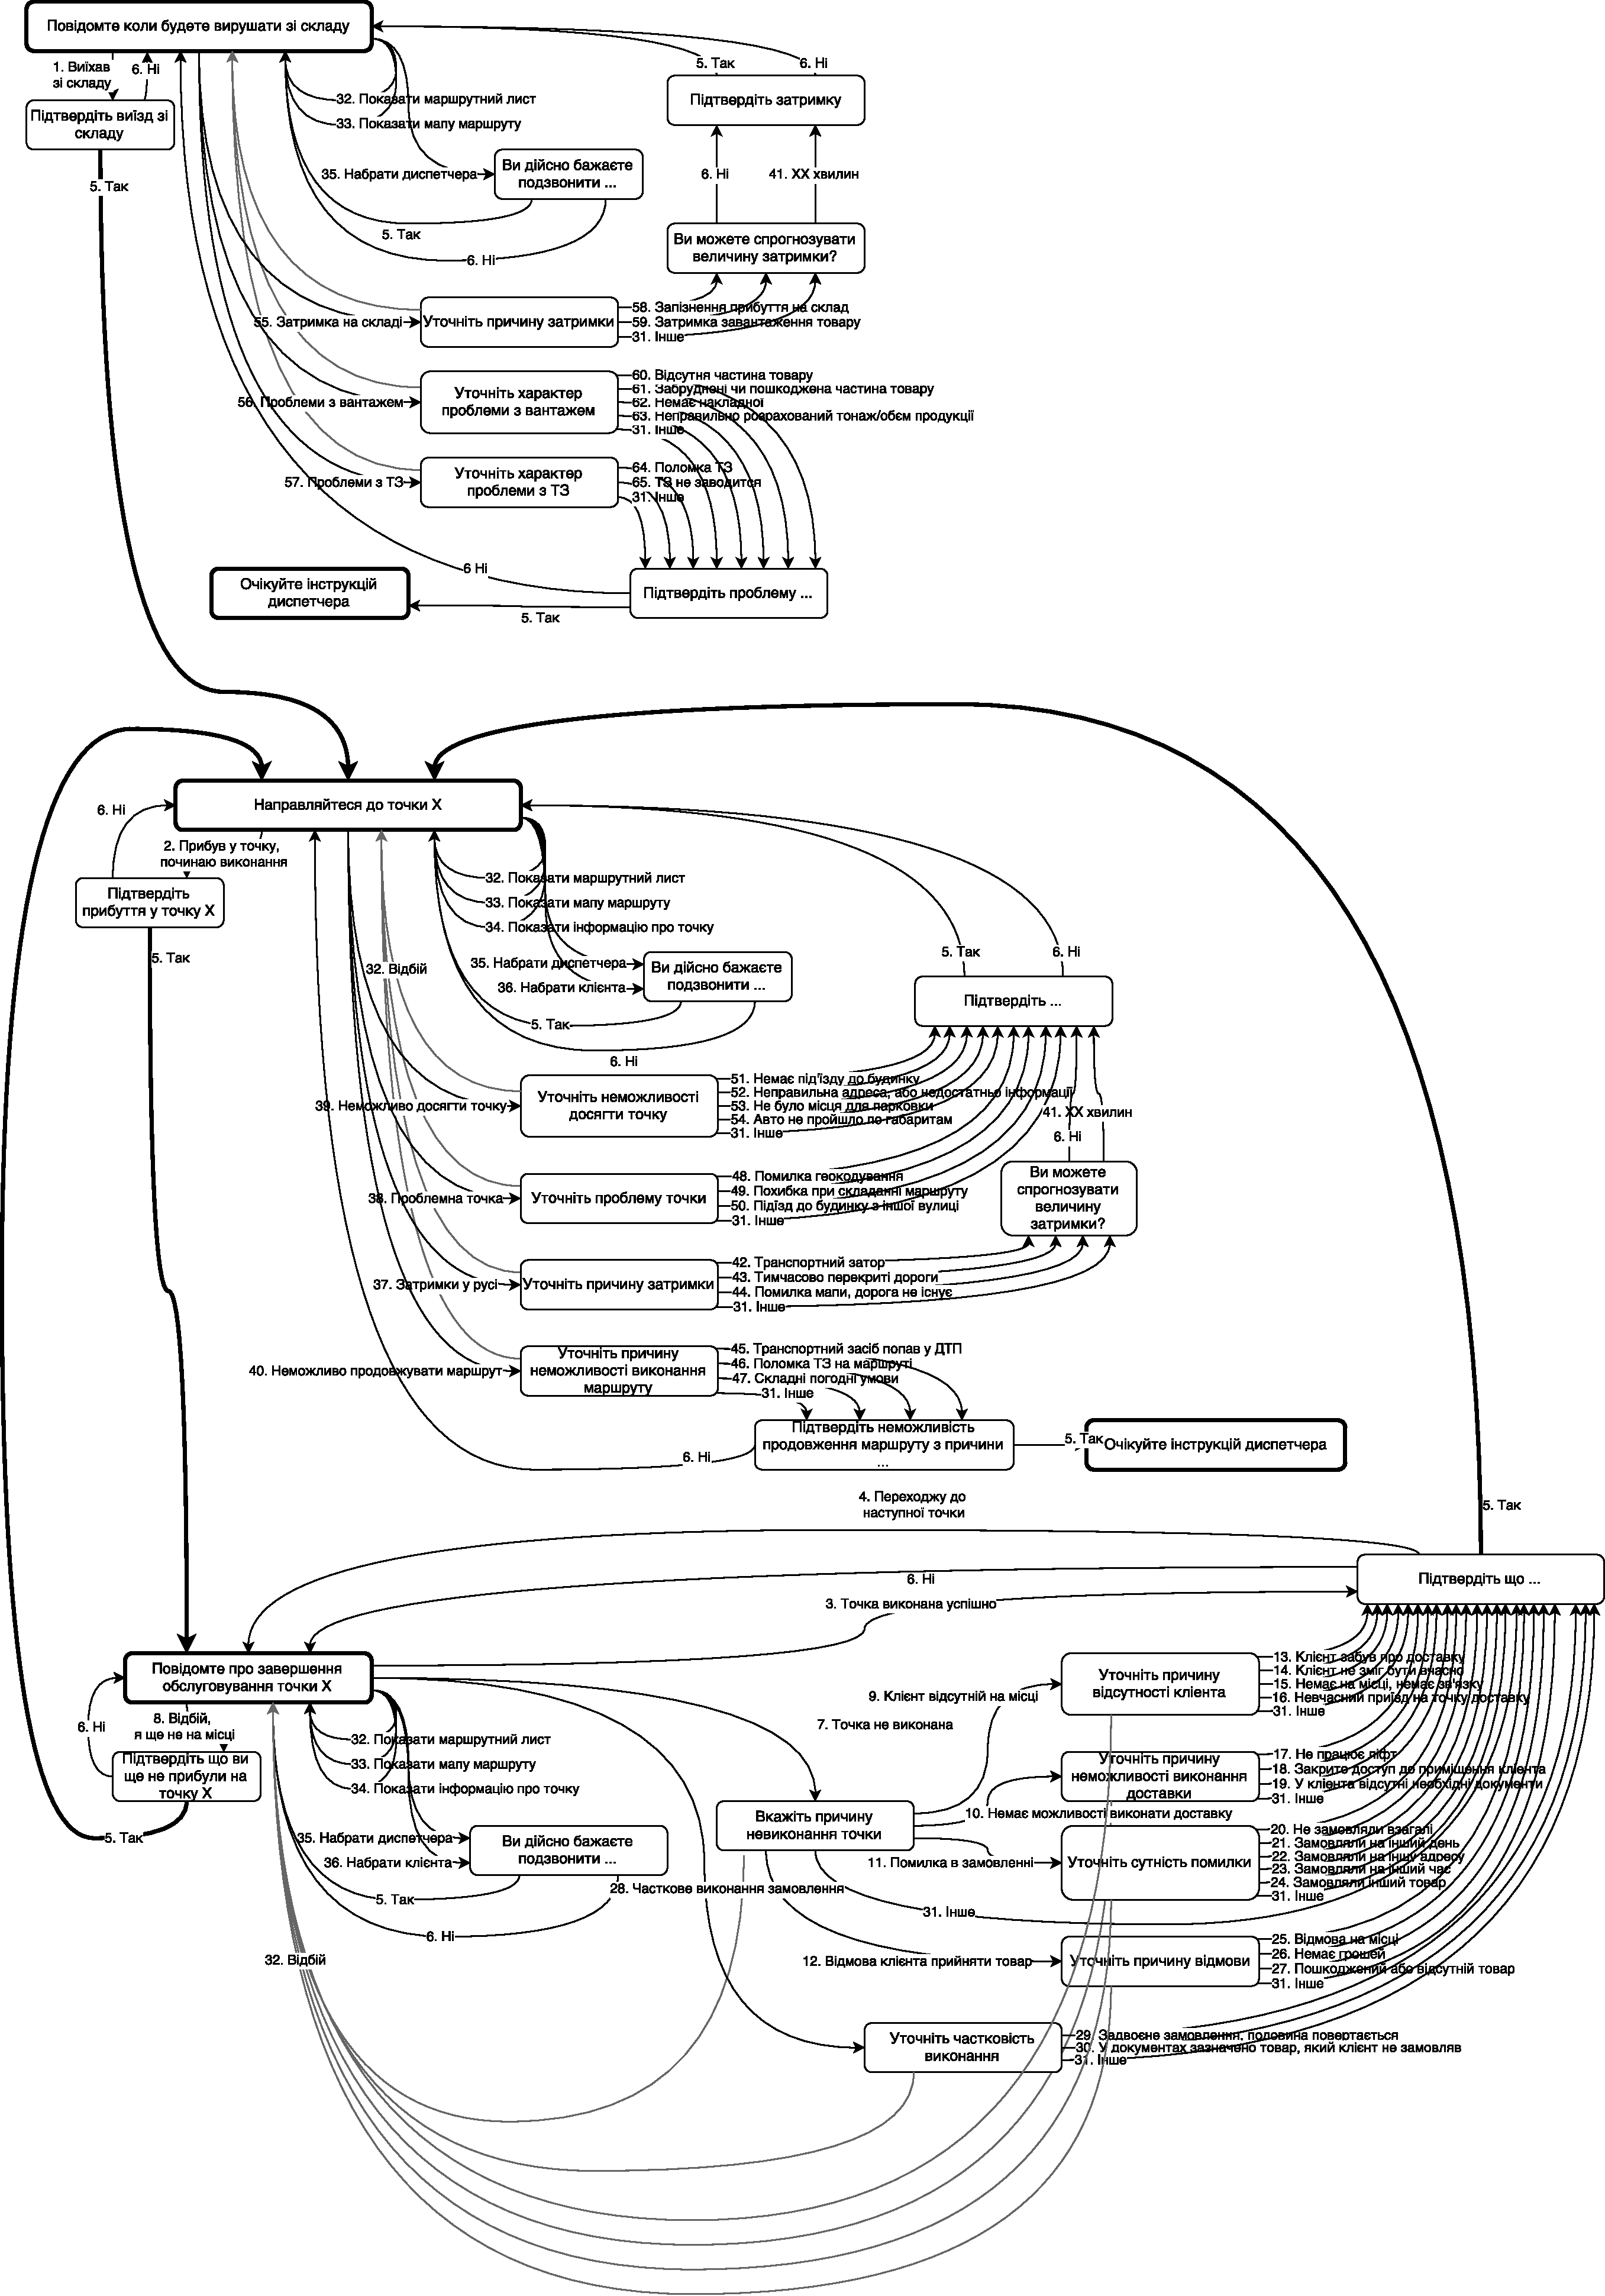
\includegraphics [width=1\linewidth] {13_complete_scenario_graph}
	\caption{Повне дерево сценаріїв всіх етапів} дистрибуції
	\label{img:13_complete_scenario_graph}
\end{figure}

\FloatBlock

У повному дереві сценаріїв усіх етапів дистрибуції (рис. \ref{img:13_complete_scenario_graph}) враховано всі можливі причини затримки або невиконання етапів «склад», «дорога», «точка доставки», а для таких випадків при неможливості виконання етапу існує вказівка (інструкції) диспетчера щодо подальших дій водія.

Наводимо повний перелік всіх унікальних стимулів з їх унікальними номерами в формі таблиці (табл. \ref{tbl:scenario_commands}).

\begin{mytable*}{ | c | l | }%
	{Різні варіанти стимулів з дерева сценаріїв}%
	{\label{tbl:scenario_commands}}%
	{№ & Варіанти стимулу}
	
	1 & Виїхав зі складу \\
	\hline
	2 & Прибув у точку, починаю виконання \\
	\hline
	3 & Точка виконана успішно \\
	\hline
	4 & Переходжу до наступної точки \\
	\hline
	5 & Так \\
	\hline
	6 & Ні \\
	\hline
	7 & Точка не виконана \\
	\hline
	8 & Відбій, я ще не на місці \\
	\hline
	9 & Клієнт відсутній на місці \\
	\hline
	10 & Немає можливості виконати доставку  \\
	\hline
	11 & Помилка в замовленні \\
	\hline
	12 & Відмова клієнта прийняти товар \\
	\hline
	13 & Клієнт забув про доставку \\
	\hline
	14 & Клієнт не зміг бути вчасно \\
	\hline
	15 & Клієнта немає на місці, немає звʼязку \\
	\hline
	16 & Невчасний приїзд на точку доставки \\
	\hline
	17 & Не працює ліфт \\
	\hline
	18 & Закрито доступ до приміщення клієнта \\
	\hline
	19 & У клиента відсутні необхідні документи \\
	\hline
	20 & Не замовляли товар взагалі \\
	\hline
	21 & Замовляли на інший день \\
	\hline
	22 & Замовляли на іншу адресу \\
	\hline
	23 & Замовляли на інший час \\
	\hline
	24 & Замовляли інший товар \\
	\hline
	25 & Відмова на місці \\
	\hline
	26 & Немає грошей \\
	\hline
	27 & Пошкоджений або відсутній товар \\
	\hline
	28 & Часткове виконання замовлення \\
	\hline
	29 & Задвоєне замовлення, половина товару повертається \\
	\hline
	30 & У документах зазначено товар, який клієнт не замовляв \\
	\hline
	31 & Інше \\
	\hline
	32 & Показати маршрутний лист \\
	\hline
	33 & Показати мапу маршруту \\
	\hline
	34 & Показати інформацію про точку \\
	\hline
	35 & Набрати диспетчера \\
	\hline
	36 & Набрати клієнта \\
	\hline
	37 & Затримки в русі \\
	\hline
	38 & Проблемна точка \\
	\hline
	39 & Неможливо дістатися точки \\
	\hline
	40 & Неможливо продовжувати маршрут \\
	\hline
	41 & \# хвилин \\
	\hline
	42 & Транспортний затор \\
	\hline
	43 & Тимчасово перекриті дороги \\
	\hline
	44 & Помилка мапи, дороги не існує \\
	\hline
	45 & Транспортний засіб потрапив у ДТП \\
	\hline
	46 & Поломка ТЗ на маршруті \\
	\hline
	47 & Складні погодні умови \\
	\hline
	48 & Помилка геокодування \\
	\hline
	49 & Похибка при складанні маршруту \\
	\hline
	50 & Підʼїзд до будинку з іншої вулиці \\
	\hline
	51 & Немає підʼїзду до будинку \\
	\hline
	52 & Неправильна адреса або недостатньо інформації \\
	\hline
	53 & Не було місця для парковки \\
	\hline
	54 & Авто не пройшло за габаритами \\
	\hline
	55 & Затримка на складі \\
	\hline
	56 & Проблеми з вантажем \\
	\hline
	57 & Проблеми з ТЗ \\
	\hline
	58 & Запізнення прибуття на склад \\
	\hline
	59 & Затримка завантаження товару \\
	\hline
	60 & Відсутня частина товару \\
	\hline
	61 & Забруднена або пошкоджена частина товару \\
	\hline
	62 & Немає накладної \\
	\hline
	63 & Неправильно розрахований тоннаж/обʼєм продукції \\
	\hline
	64 & Поломка ТЗ \\
	\hline
	65 & ТЗ не заводится \\
\end{mytable*}

Модель голосової взаємодії субʼєктів дистрибуції може бути представлена у вигляді орієнтовного графу $G$, що складається з множини вершин $V$ та множини ребер $E$:

\begin{align}
	G&=\langle V,E\rangle; \nonumber\\
	E&=\{\langle v_i,v_j\rangle | v \in V\}. \nonumber
\end{align}

При цьому існує відношення $f_R$ множини ребер до множини реакцій та відношення $f_C$ множини вершин до множини контекстів, такі що:

\begin{align}
	f_R&: E \rightarrow R,\quad R\subset\mathbb{N},\quad |R|\le|E|; \nonumber\\
	f_C&: V \rightarrow C,\quad C\subset\mathbb{N},\quad|C|\le|V|; \nonumber\\
	R_V(v_i) &= \{f_R(e)|\forall j:e=\langle v_i,v_j\rangle \in E\}; \nonumber\\
	\forall i,j: f_C(v_i)&=f_C(v_j) \iff R_V(v_i) = R_V(v_j), \nonumber
\end{align}

\noindent
де $R_V(v_i)$ --- множина реакцій, можливих у вершині $v_i$.

Адекватність розробленої моделі підтверджується її повною відповідністю статистичним даним інцидентів, зібраних за період упровадження системи, та експериментально --- шляхом порівняння результатів моделювання з використанням моделі та без її залучення.

\subsection{Виділення унікальних контекстів моделі голосової взаємодії}

Як було зазначено в підрозділі \ref{sect2_3}, кожна вершина в орієнтованому графі сценаріїв голосової взаємодії водія в системах диспетчерського контролю за рухом автотранспорту (рис. \ref{img:13_complete_scenario_graph}) позначає контекст голосової взаємодії, який може бути змодельовано окремо, а перелік ребер, що виходять з цієї вершини, обмежує можливий перелік голосових команд, які мають  бути розпізнані в цьому контексті.

Оскільки деякі контексти мають однаковий перелік можливих голосових команд, можемо не створювати для кожного з таких контекстів окрему модель, а повторно використовувати вже існуючі моделі контекстів з тим самим переліком голосових команд. Для визначення переліку необхідних моделей пронумеруємо всі контексти, представлені на дереві сценаріїв, залежно від переліку команд, які в них можуть бути розпізнані.

Повне дерево сценаріїв усіх етапів дистрибуції «склад – дорога – точка доставки» з вказівкою контекстів наведено на рис. \ref{img:14_complete_scenario_graph_contexts}. Використовуємо повне дерево сценаріїв, щоб знайти і пронумерувати унікальні контексти.

\begin{figure}
	\centering
	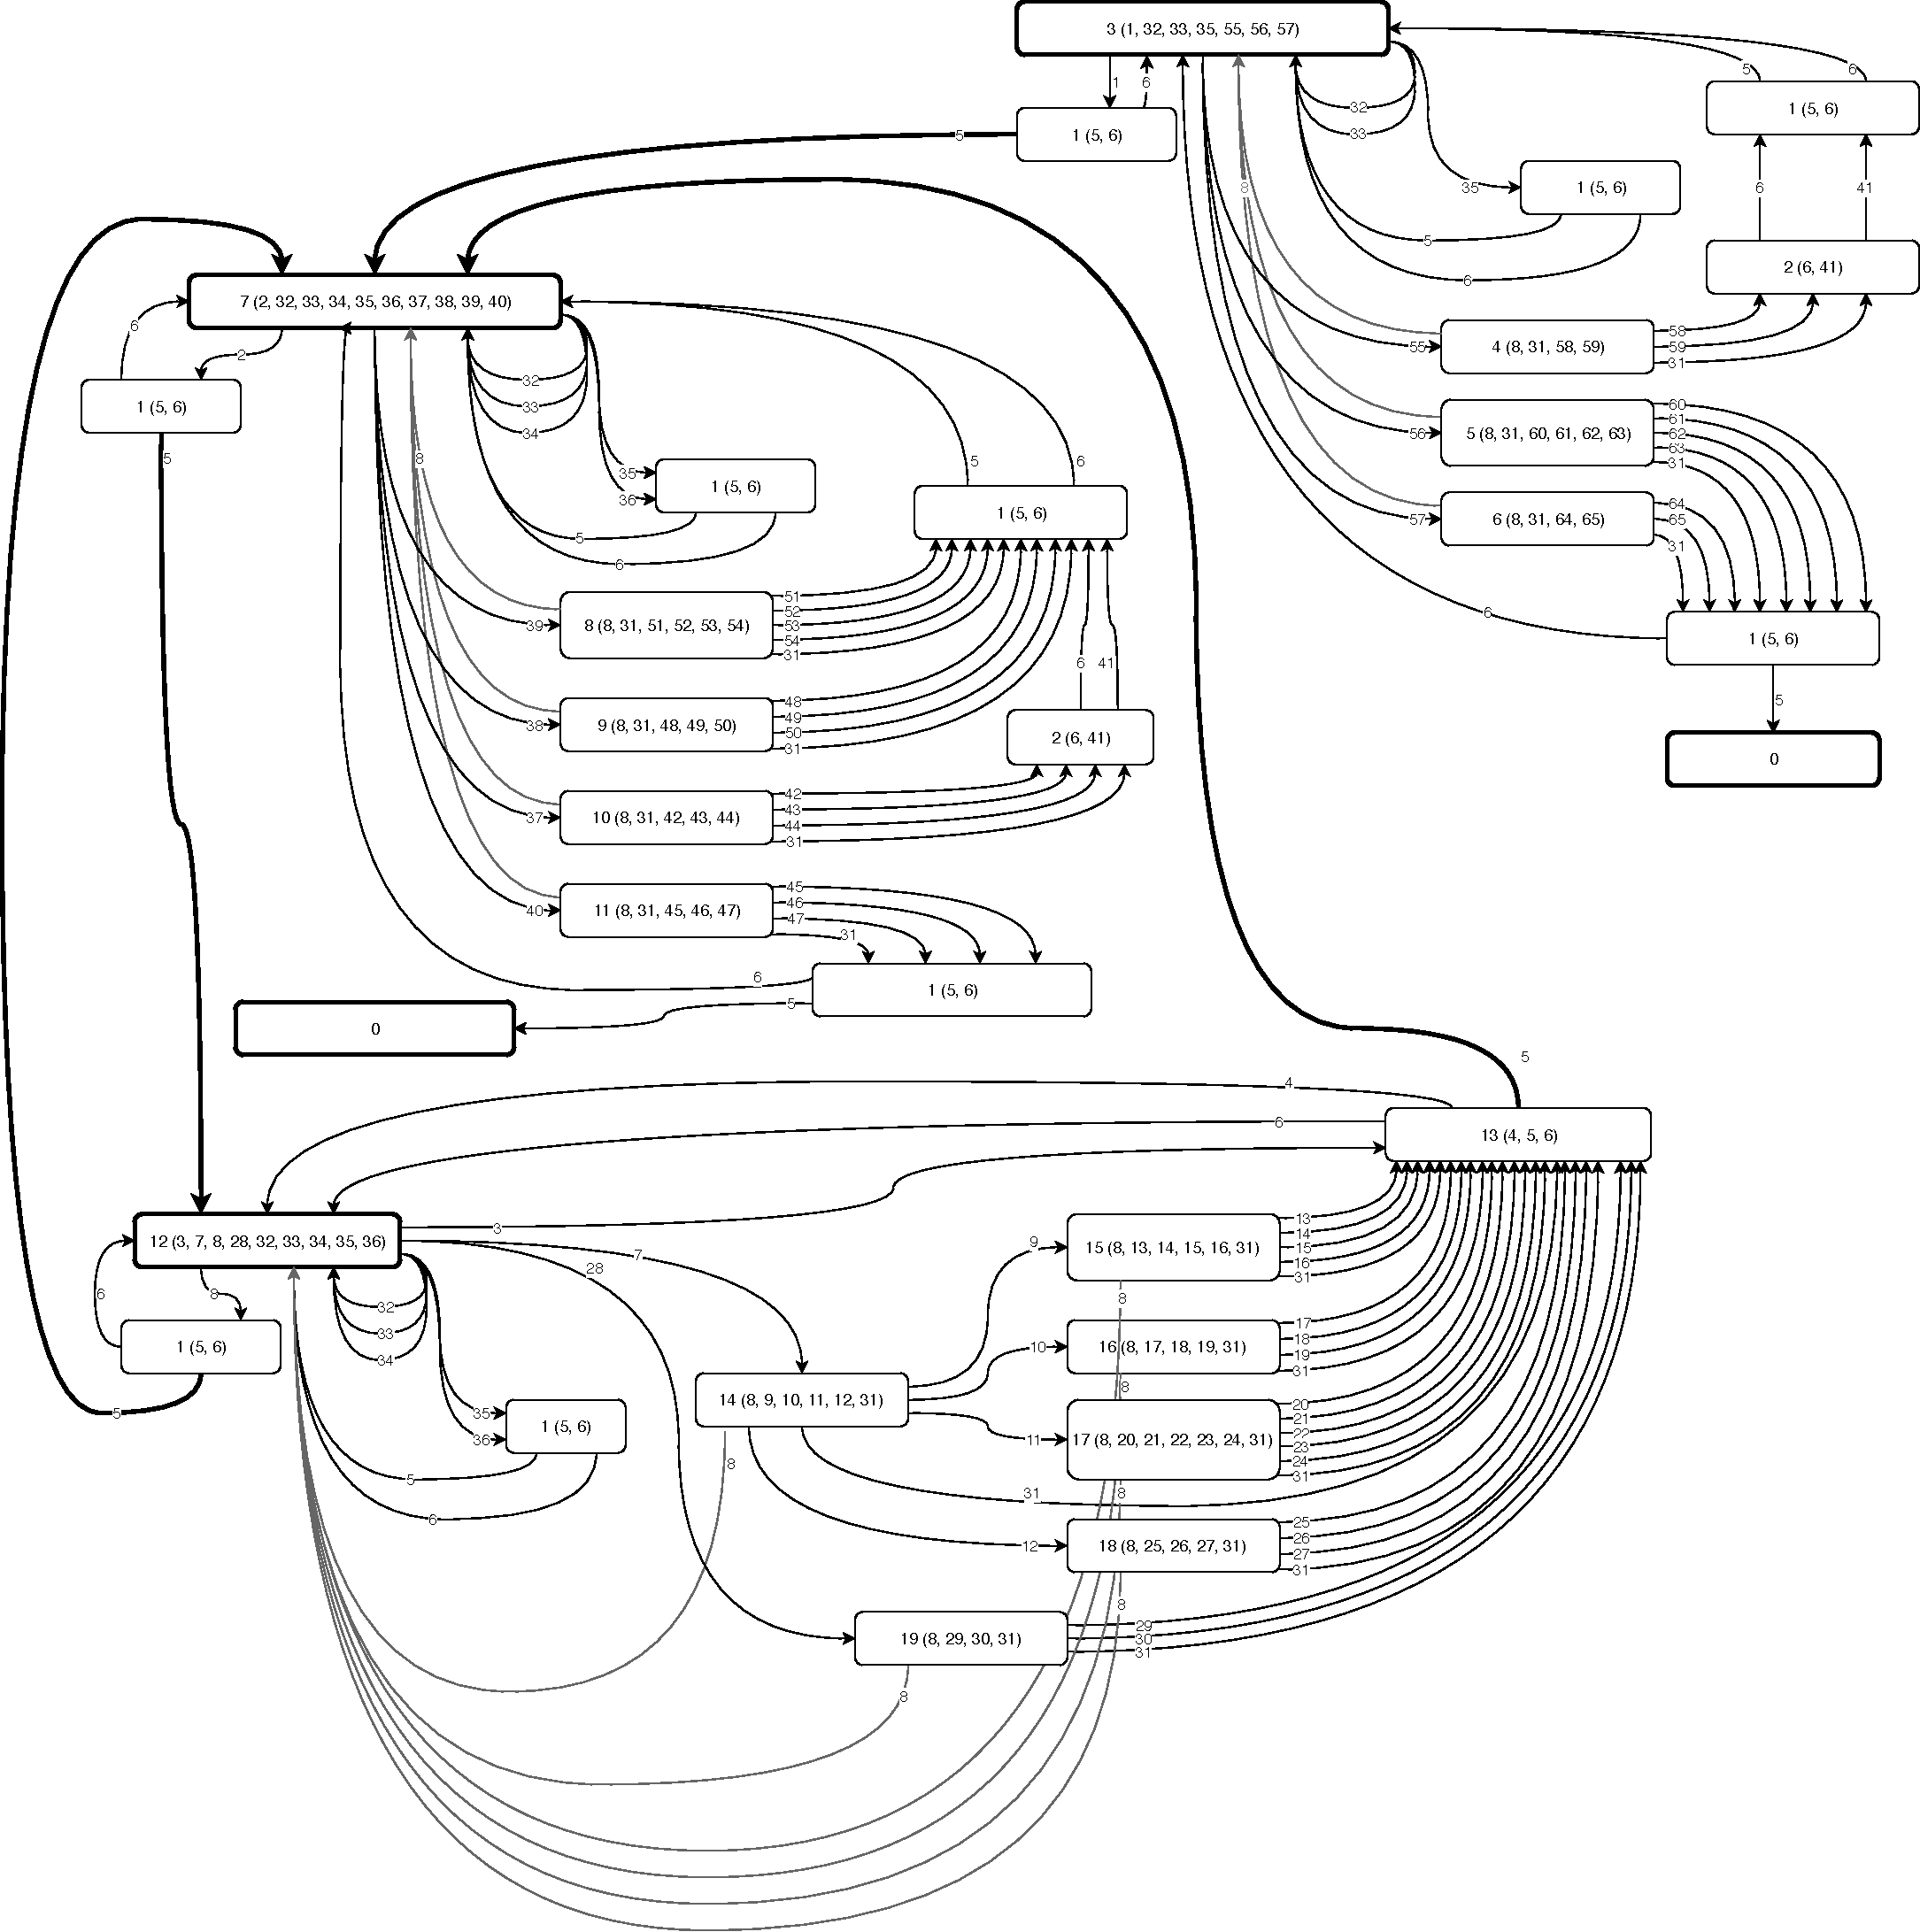
\includegraphics [width=1\linewidth] {14_complete_scenario_graph_contexts}
	\caption{Повне дерево сценаріїв усіх етапів дистрибуції з указанням контекстів}
	\label{img:14_complete_scenario_graph_contexts}
\end{figure}

Повне дерево сценаріїв усіх етапів дистрибуції «склад – дорога – точка доставки» з вказівкою контекстів (рис. \ref{img:14_complete_scenario_graph_contexts}) містить можливі реакції в них, тобто на кожний позначений контекст (табл. \ref{tbl:scenario_commands}) існує реакція, яку вказано в дужках на дереві сценаріїв.

У табл. \ref{tbl:context_reactions} представлено звʼязок контекстів і реакцій на них в моделі голосової взаємодії водія в системі диспетчерського контролю за рухом автотранспорту.

Відповідно до наведених блоків контексту в моделі голосової взаємодії водія в системі диспетчерського контролю за рухом автотранспорту прослідковується звʼязок можливих реакцій на них. Отже, відповідно до цього можна будувати систему формалізації голосової інформації.

\begin{mytable}{ | c | l | }%
	{Перелік контекстів та можливих реакцій у них}%
	{\label{tbl:context_reactions}}%
	{№ & Можливі реакції}
	
	1 & 5, 6 \\
	\hline
	2 & 6, 41 \\
	\hline
	3 & 1, 32, 33, 35, 55, 56, 57 \\
	\hline
	4 & 8, 31, 58, 59 \\
	\hline
	5 & 8, 31, 60, 61, 62, 63 \\
	\hline
	6 & 8, 31, 64, 65 \\
	\hline
	7 & 2, 32, 33, 34, 35, 36, 37, 38, 39, 40 \\
	\hline
	8 & 8, 31, 51, 52, 53, 54 \\
	\hline
	9 & 8, 31, 48, 49, 50 \\
	\hline
	10 & 8, 31, 42, 43, 44  \\
	\hline
	11 & 8, 31, 45, 46, 47 \\
	\hline
	12 & 3, 7, 8, 28, 32, 33, 34, 35, 36 \\
	\hline
	13 & 4, 5, 6 \\
	\hline
	14 & 8, 9, 10, 11, 12, 31 \\
	\hline
	15 & 8, 13, 14, 15, 16, 31 \\
	\hline
	16 & 8, 17, 18, 19, 31 \\
	\hline
	17 & 8, 20, 21, 22, 23, 24, 31 \\
	\hline
	18 & 8, 25, 26, 27, 31 \\
	\hline
	19 & 8, 29, 30, 31 \\
\end{mytable}

\subsection{Створення моделі формалізації голосової інформації для кожного контексту голосової взаємодії}

Розглянемо будь-який контекст голосової взаємодії водія в системах диспетчеризації автотранспорту. Для формалізації голосової інформації в цьому контексті необхідно створити модель класифікації голосових висловлювань водія, що відповідає можливому переліку голосових команд у моделі голосової взаємодії.

Представимо перелік можливих голосових команд як множину:

\[
A = {A_i | i=\overline{1..n}},
\]

\noindent
де $A$ --- множина голосових команд $A_i$, а $n$ --- кількість можливих голосових команд у контексті, що розглядається.

Тоді для кожного голосового висловлювання $B$, сказаного водієм, існує ймовірність $p(A_i/B)$, що це висловлювання було командою $A_i$. Задача формалізації голосової інформації полягає у визначенні того, яка з команд є найбільш ймовірною.

Для вирішення цієї задачі пропонується дуальна система класифікації, яка може бути налаштована на предметну область і використовувати метод інтелектуальних рефлекторних систем або метод згорткових нейронних мереж залежно від того, який з них показує кращі результати.

У даному підрозділі представлено розроблене дерево сценаріїв усіх етапів дистрибуції «склад – дорога – точка доставки» як модель голосової взаємодії водія в системах диспетчерського контролю за рухом автотранспорту та визначено перелік контекстів та можливих реакцій на них.

\section{Дуальний метод формалізації голосової інформації в системах диспетчерського контролю за рухом автотранспорту} \label{sect3_4}

\subsection{Інтелектуальні рефлекторні системи}

Для формалізації голосової інформації можна використати систему з двох основних модулів: автоматичного фонетичного стенографа і ядра рефлекторної системи голосового управління (РСГУ), поточна реалізація яких визначає умови їх використання в моделі голосової взаємодії водія при диспетчерському контролі за рухом автотранспорту (рис. \ref{img:rsgu_struct}).

\begin{figure}
	\centering
	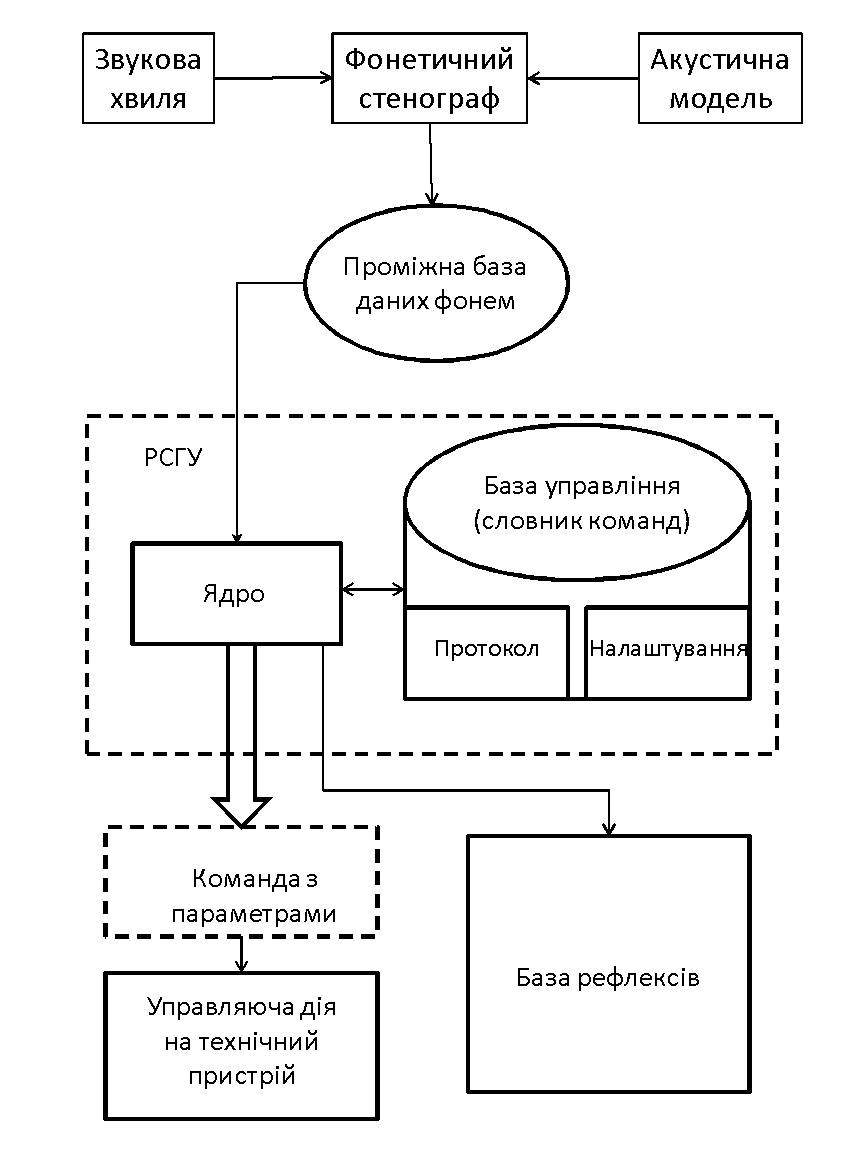
\includegraphics [width=.5\linewidth] {rsgu_struct}
	\caption{Структура системи формалізації голосової інформації в моделі голосової взаємодії водія при диспетчерському контролі за рухом автотранспорту}
	\label{img:rsgu_struct}
\end{figure}

Застосування алгоритму фонетичного стенографа дає змогу будувати послідовність контекстів для мовного сигналу без використання будь-якого словника. З цією метою будується деяка генеративна граматика, яка може синтезувати всі можливі модельні сигнали безперервної мови для будь-якої послідовності фонем. У межах побудованої моделі розробляється алгоритм пофонемного розпiзнавання для невідомого сигналу з використанням контекстів та можливих реакцій на них.

Виконання фонетичного стенографу \cite{Pylypenko_2008} здійснено у вигляді бінарного додатку, набору бібліотек і конфігураційних файлів для платформи Windows, а саме ядро РСГУ, яке виконує реалізацію інтроформаційного методу вироблення рефлексів, розроблено і виконано в середовищі MS Access на всіх операційних системах сімейства Windows.

У системі формалізації голосової інформації, що розглядається (рис. \ref{img:rsgu_struct}), вхідною інформацією виступає голосова команда, яка може бути представлена звуковою хвилею; вихідною ж інформацією виступатиме процес керуючого впливу на обʼєкт управління, тобто відбуватиметься виконання розпізнаної команди відповідно до попередньо заданих голосом параметрів.

Сама система формалізації голосової інформації в процесі роботи генеруватиме потрібні візуальні і голосові інформаційні повідомлення водію, а це, у свою чергу, надаватиме можливість відслідковувати процес розпізнавання команд, реакції на них і, крім того, даватиме змогу в реальному масштабі часу змінювати поведінку системи в разі потреби.

Розглянемо схему роботи системи формалізації голосової інформації в моделі голосової взаємодії водія при диспетчерському контролі за рухом автотранспорту. Водій у вільній формі озвучує необхідні для нього дії системи. Наприклад, по відношенню до голосового управління системою це може бути: «Показати маршрутний лист», або «Показати мапу маршруту», або «Показати інформацію про точку». Програмна платформа системи формалізації голосової інформації в моделі голосової взаємодії водія при диспетчерському контролі за рухом автотранспорту передає необхідну команду на технічний пристрій або озвучує водієві затребувану  ним  інформацію. Під час  навчання водій сам виконує відповідну дію і у системи виробляється рефлекс на подібне звернення. Якщо водії говорять «по-різному», то виробляється стійкий рефлекс саме на інформативну частину голосової команди. При цьому в системі формалізації голосової інформації в моделі голосової взаємодії водія при диспетчерському контролі за рухом автотранспорту наявні такі стани, команди та засоби:

1. \textbf{Звукова команда}. Водій голосом звертається з проханням до технічного пристрою.

Вихідною інформацією є звукова хвиля.

Наведемо приклад для даної команди: покажи мені, будь ласка, інформацію про точку.

2. \textbf{Акустична модель}. Включає статистичний опис розпізнавання мови і особливостей мови водія. Статистичний опис формується в процесі навчання налаштуванням на водіїв. Як акустичні використовуються приховані Марківські моделі. 65 українських контекстно-незалежних фонем моделюються трьома станами Марківського ланцюга без пропуску.

Створення словника транскрипцій акустичних моделей відбувається автоматично з орфографічного словника з використанням контекстно-незалежних правил.

3. \textbf{Фонетичний стенограф}. Служить для перетворення вхідного оцифрованого звукового сигналу, що містить усне мовлення (акустичної моделі), в набір фонем.

Алгоритм фонетичного стенографа дає змогу будувати послідовність фонем для мовного сигналу без використання будь-якого словника. З цією метою будується деяка генеративна граматика, яка може синтезувати всі можливі модельні сигнали безперервної мови для будь-якої послідовності фонем. У межах побудованої моделі розробляється алгоритм пофонемного розпiзнавання для невідомого сигналу. Використовуються ті самі контекстно незалежні моделі фонем, як і в базовому розпізнавачі.

Надійність виявлення фонеми на правильному місці для відомої реалізації дорівнює приблизно 70\%.

Вихідна інформація: проміжна база даних фонем – результат розпізнавання вхідних звукових хвиль.

4. \textbf{Ядро РСГУ}. Призначено для моделювання системи голосового управління технічним пристроєм. Містить програмну реалізацію інтроформаційного методу, а також алгоритмів виділення комбінацій фонем і навчання (накопичення статистики). Інформаційна база управління містить словник команд, протокол роботи, налаштування системи.

5. \textbf{Команда з параметрами}. Результатом роботи системи є команда з параметрами, яку необхідно реалізувати технічному пристрою.

Вихідною інформацією є виконувана команда.

Приклад: водій – Найдьонов, команда – Х хвилин, рівень – десятки, десятки хвилин – 10, одиниці хвилин – 8.

6. \textbf{Керуючий вплив}. Містить програмну реалізацію алгоритму управління технічним пристроєм.

Вхідною інформацією є формалізована команда з відповідними параметрами.

Результатом керуючого впливу є зміна параметрів самого технічного пристрою.

Прикладом керуючого впливу може бути інформація про наступний час виконання.

Система формалізації голосової інформації в моделі голосової взаємодії водія при диспетчерському контролі за рухом автотранспорту відрізняється простотою і, в даному випадку, реалізує рефлекторну модель поведінки, яку наведено на рис. \ref{img:rsgu_scheme}

\begin{figure}
	\centering
	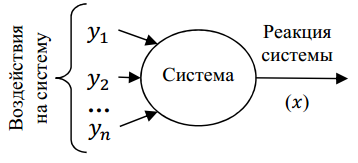
\includegraphics [width=.5\linewidth] {rsgu_scheme}
	\caption{Схема реакції системи формалізації голосової інформації в моделі голосової взаємодії водія при диспетчерському контролі за рухом автотранспорту на несилові впливи}
	\label{img:rsgu_scheme}
\end{figure}

Система формалізації голосової інформації в моделі голосової взаємодії водія при диспетчерському контролі за рухом автотранспорту функціонує в режимі навчання і режимі управління. У режимі навчання відбувається формування бази рефлексів.
У режимі управління РСГУ відбувається вироблення реакції на звернення водія. Також у цьому режимі відбувається реалізація режиму самонавчання – для випадку, коли отримана реакція не задовольняє водія.

Основною частиною системи формалізації голосової інформації в моделі голосової взаємодії водія при диспетчерському контролі за рухом автотранспорту є база рефлексів. База рефлексів містить статистику вхідних впливів (комбінацій фонем) і реакцій системи, розділених на класи: водій, команда, рівень числа, десятки, одиниці (рис. \ref{img:rsgu_base}).

\begin{figure}
	\centering
	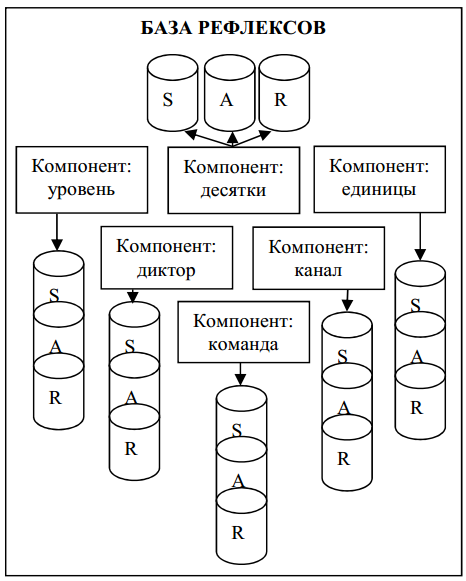
\includegraphics [width=.5\linewidth] {rsgu_base}
	\caption{Структура бази рефлексів системи формалізації голосової інформації}
	\label{img:rsgu_base}
\end{figure}

Реалізація кожного класу рефлексів відбувається в кожному окремому компоненті системи формалізації голосової інформації в моделі голосової взаємодії водія при диспетчерському контролі за рухом автотранспорту. Представлення кожного компоненту системи здійснюється у вигляді окремого «інтроформаційного» нейрона.

На вході системи задається повний вхідний набір фонем та/або реакція інших «інтроформаційних» нейронів, на виході – вироблена реакція нейронів, яка надходить на інші «інтроформаційні» нейрони або безпосередньо на технічний пристрій.

У кожному компоненті системи формалізації голосової інформації в моделі голосової взаємодії водія при диспетчерському контролі за рухом автотранспорту інформація зберігається в таких таблицях:

\begin{itemize}
	\item S – таблиця з комбінацією фонем, в якій знаходяться та зберігаються всі комбінації послідовних фонем з довжинами від 2-х до 10 символів з інформацією про те, скільки разів вони траплялися;
	\item R – таблиця реакції РСГУ, в якій міститься перелік дій, які необхідно виконати РСГУ або технічному пристрою, частота користування і визначеність даної реакції. Реакція типу «Не знаю» забезпечує відкритість системи;
	\item А – таблиця, призначена для встановлення звʼязку вищенаведених таблиць S і R. Містить інформацію про те, яка реакція і скільки разів була затребувана у випадку, коли на вході був деякий набір фонем. Крім того, таблиця містить відомості про визначеність реакції, що повʼязана з цим набором фонем.
\end{itemize}

При режимі навчання у вищенаведених таблицях відбувається накопичення інформації про звʼязок вхідних фраз (контекстів) і реакцій системи формалізації голосової інформації в моделі голосової взаємодії водія при диспетчерському контролі за рухом автотранспорту. У процесі роботи системи отримана інформація використовується далі в режимі управління для вироблення реакцій на відповідні звернення водія на основі інтроформаційного методу \cite{Teslia_2010}. При цьому алгоритм реалізації режиму управління в системі має таку послідовність:

\begin{itemize}
	\item перший етап. Старт алгоритму.
\end{itemize}

При надходженні на вхід системи потоку фонем виділяються фрагменти (набори) множиною M, що містять від 2 до 4 символів, які стоять поруч;

\begin{itemize}
	\item другий етап. Відбір класу команд.
\end{itemize}

З таблиці S здійснюється відбір записів, які відповідають сформованим наборам фонем, що належать до множини M.
На основі інтроформаційного методу відбувається обчислення визначеності реакцій (команд), що містяться в таблицях A і R. Команда, що має найбільшу визначеність, вибирається для реалізації;

\begin{itemize}
	\item третій етап. Якщо в команді є звернення до числового значення (знак \#), розглядаються класи рівня числа (десятки, одиниці).
\end{itemize}

Клас рівня числа. З таблиці S здійснюється відбір записів, які відповідають сформованим наборам фонем (що входять у множину M). З використанням таблиць A і R відповідно до інтроформаційного методу обчислюється визначеність рівня числа. Варіанти: немає десятків хвилин (числа від 0 до 9), є десятки хвилин (числа більше 9).

Якщо рівень числа «Є десятки хвилин», то активізуються таблиці, що входять у клас десятків хвилин. З таблиці S здійснюється відбір записів, які відповідають сформованим наборам фонем (що входять у множину M). З використанням таблиць A і R відповідно до інтроформаційного методу обчислюється визначеність номера десятка. Якщо десяток не визначений, у команду вставляється знак «?».

Клас одиниць хвилин. З таблиці S здійснюється відбір записів, які відповідають сформованим наборам фонем (що входять в множину M). Використовуючи таблиці A і R, відповідно до інтроформаційного методу обчислюється визначеність другий цифри в числі. Якщо цифра не визначена, в команду вставляється знак «?»;

\begin{itemize}
	\item четвертий етап. Завершення алгоритму.
\end{itemize}

Отже, метод інтелектуальних рефлекторних систем для формалізації голосової інформації в системах диспетчерського контролю за рухом автотранспорту можна представити таким чином:

\begin{enumerate}
	\item запис фрази, вимовленої водієм; $A_i=<a_1,a_2,...,a_n>; t=\frac{n}{s}; s=16 \textbf{(kHz)};$
	\item перетворення записаної фрази на фонетичний текст за допомогою фонемного стенографа; $P_i=S(A_i); P=<p_1,p_2,...,p_k>; p_i \in F;$
	\item класифікація фонемної репрезентації голосової команди; $y_i=C_c(P_i)$
	\begin{enumerate}
		\item розбиття фонетичного тексту на N-грами фонем різної довжини;
		\item розрахунок інтроформаційного впливу кожного N-граму фонем на можливі команди у вибраному контексті;
		\item вибір команди з найбільшою ймовірністю;
	\end{enumerate}
	\item виконання відповідної реакції (озвучення відповіді, виконання команди та/або відправка структурованих даних диспетчеру);
	\item переключення контексту на новий, відповідний до вибраної реакції; $c_{i+1} = f(c_i, y_i)$
	\item очікування та запис наступної фрази.
\end{enumerate}

{\settowidth{\leftskip}{Де:\ }
	
	$A_i$ --- цифровий аудіозапис команди водія довжиною $t$ секунд,
	
	$n$ --- кількість семплів аудіосигналу,
	
	$s$ --- частота дискретизації аудіосигналу,
	
	$P_i$ --- представлення команди водія у вигляді фонемного тексту --- кортежу фонем довжини $k$,
	
	$F$ --- множина фонем української мови,
	
	$S$ --- фонемний стенограф,
	
	$y_i$ --- реакція з моделі голосової взаємодії субʼєктів дистрибуції, яка відповідає вимовленій команді,
	
	$C_c$ --- класифікатор фонемної репрезентації голосових команд відповідно до поточного контексту $c_i$,
	
	$f$ --- функція визначення наступного контексту залежно від поточного контексту $c_i$ та вибраної реакції $y_i$.
	
}

Таким чином, у кожний компонент системи надходить весь вхідний набір фонем без виділення слів, команд, пропозицій тощо. Результат роботи даного методу такий самий, як і роботи головного мозку людини. Тобто, слухаючи усне мовлення, або читаючи лист, людина, не виокремлюючи букви і слова, розпізнає сенс. Те саме відбувається і в рефлекторній системі голосового управління. При цьому не потрібно створювати ніяких словників, виконувати морфологічний, синтаксичний, семантичний аналіз тексту, а також виділяти слова і команди; виникнення реакції відбувається на звуковий потік, з якого система формалізації голосової інформації в моделі голосової взаємодії водія при диспетчерському контролі за рухом автотранспорту, як і людина, сама «вміє виділяти» інформативну частину за максимальною визначеністю \cite{Teslia_2013}.

Для підвищення ефективності розпізнавання було запропоновано удосконалену схему системи формалізації голосової інформації в моделі голосової взаємодії водія в дистрибуції (рис. \ref{img:rsgu_struct_new}), яка включає моделювання за кожним контекстом із моделі голосової взаємодії та дуальну систему класифікації фонемної репрезентації голосових команд, що дає змогу вибрати кращий метод класификації залежно від предметної області.

\begin{figure}[h!]
	\centering
	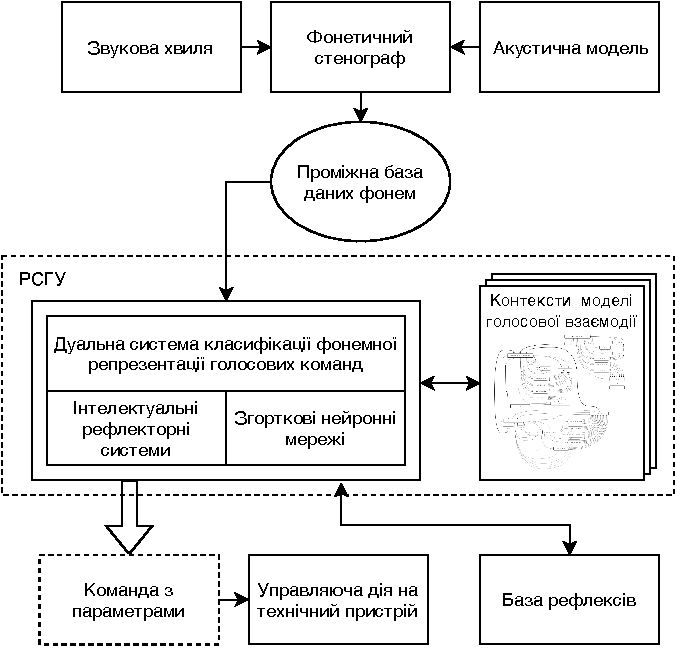
\includegraphics [width=.6\linewidth] {rsgu_struct_new}
	\caption{Удосконалена схема системи формалізації голосової інформації в моделі голосової взаємодії водія при диспетчерському контролі за рухом автотранспорту}
	\label{img:rsgu_struct_new}
\end{figure}

У якості альтернативного класифікатора фонетичного тексту голосової команди запропоновано використання методу згорткових нейронних мереж, що широко використовується в різноманітних задачах класифікації звукових даних \cite{Weisskirchen_2017,Boddapati_2017,Chowdhury_2018} та природномовних текстів \cite{Kim_2014,Britz_2015_2,Britz_2015,Kim_2016,Zhang_2015_2,Zhang_2015,Santos_2014}.

\subsection{Згорткові нейронні мережі}

У даному випадку система формалізації голосової інформації в моделі голосової взаємодії водія при диспетчерському контролі за рухом автотранспорту аналогічно до РСГУ, складається з двох частин: фонемний стенограф та сама згорткова нейронна мережа (ЗНМ), яка працює з фонемами.
ЗНМ для роботи з фонемами найбільше нагадує ЗНМ у задачі класифікації текстів \cite{Kim_2014}, але працює з «текстом» не по словах, а пофонемно, що схоже на роботу з текстом посимвольно \cite{Zhang_2015}.

ЗНМ дуже схожі на звичайні нейронні мережі: вони також побудовані на основі нейронів, які характеризуються постійно змінюваною вагою і зсувами. Кожен нейрон отримує деякі вхідні дані, виконує скалярне перетворення інформації і, в окремих ситуаціях, супроводжується нелінійністю. Як і у випадку зі звичайними нейронними мережами, вся ЗНМ моделює одну диференційовану функцію внеску: з одного боку, це необроблені фонеми, з іншого – висновок щодо класу або групи ймовірних класів, які характеризують фонему. Також наявна функція втрати на останньому (повністю підключеному) шарі ЗНМ.

Архітектура ЗНМ робить явне припущення виду «вхідні дані є фонеми», що дає змогу закодувати певні властивості під архітектуру. Завдяки цій особливості попереднє оголошення можна реалізувати більш ефективно, зменшуючи при цьому кількість параметріу в мережі.

Нейронні мережі отримують вхідні дані (один вектор), після чого трансформують інформацію, проводячи її через ряд прихованих шарів \cite{Kim_2014, Zhang_2015}. Кожен прихований шар складається з множини нейронів, де всякий нейрон має стійкий звʼязок з усіма нейронами в попередньому шарі і де нейрони в функції одного шару повністю незалежні один від одного і не мають спільних звʼязків. Останній повнозвʼязний шар називається вихідним шаром і в налаштуваннях класифікації він демонструє число класів.

На відміну від звичайних повнозвʼязних нейронних мереж, згорткові нейронні мережі враховують просторову структуру даних, тобто, той факт, що фонеми, які знаходятся поряд, мають більший звʼязок між собою і спільний вплив на результуючу змінну.

У роботі, за основу реалізації було взято реалізацію з відкритим вихідним кодом \cite{Britz_2015} на мові Python з використанням TensorFlow.

Структура нейронної мережі може бути представлена у такий спосіб (рис. \ref{img:cnn-struct}).

\begin{figure}
	\centering
	\subbottom[\label{img:cnn-struct1}]{%
		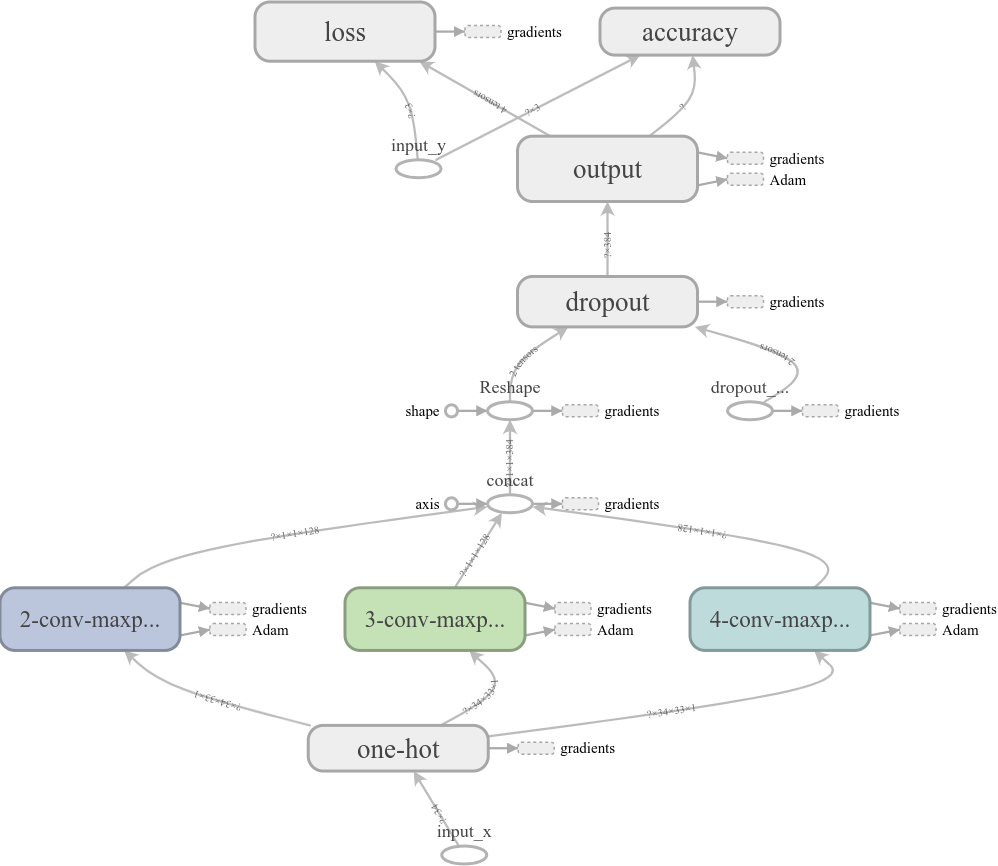
\includegraphics[width=.7\linewidth]{cnn_1}}
	\hfill
	\subbottom[\label{img:cnn-struct2}]{%
		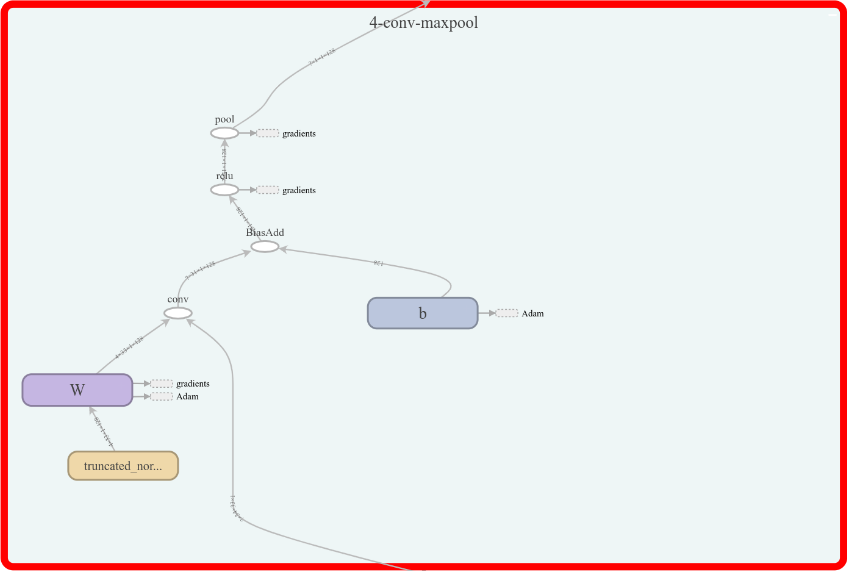
\includegraphics[width=.25\linewidth]{cnn_2}}
	\caption{Структура згорткової нейронної мережі (\subcaptionref{img:cnn-struct1}) та деталізація її згорткового шару (\subcaptionref{img:cnn-struct2})}
	\label{img:cnn-struct}
\end{figure}

Фонеми представлено у вигляді one-hot вектору. Фрази нормалізовано за максимальною довжиною з використанням вектора з усіма нулями в якості заповнювача.

На відміну від випадку роботи за словами, у ЗНМ класифікації фонем вкладений шар (embedding layer) відсутній, оскільки потужність множини фонем набагато нижча, ніж потужність множини слів, що робить такий шар не необхідним. З іншого боку, деякі фонеми схожі на інші, деякі --- ні, тому використання вкладень може бути доцільним для передачі цієї схожості, а не тільки для зниження розмірності. Навчання вкладеного шару потребує великого обʼєму вхідних даних, тому в даній роботі розглядатися не буде.

Використовується комбінований згортковий шар (convolution layer), який складається з кількох паралельних одновимірних шарів з різними варіантами кроку фільтра.

Для агрегації кожного зі згорткових шарів використовується агрегаційний шар (pooling layer) з вибором одного максимального значення (1-max-pooling).

Виходи агрегаційних підшарів різного розміру кроку згортки комбінуються в один вектор значень.

У якості повнозвʼязного шару використовується класичний перцептрон, який може мати активаційну функцію у вигляді не спадаючих диференційованих функцій, що діють на множині дійсних чисел. У нашому випадку для функції активації використаємо ReLU:

\[
h(a) = \max(0, a),
\]

\noindent
де $a=WX+b$

Застосування у якості функції активації ReLU дозволяє забезпечити головні переваги, які надають можливість здійснити пришвидшення навчання нейронної мережі через розрідженість та меншу величину ймовірності розмиття градієнту порівняно з іншими активаційними функціями. Виникнення розрідженості відбувається при значеннях a < 0. Для більшої кількості нейронів з ReLU-активацією в шарі характерна більша розрідженість отриманого результату.

Для зниження ефекту перенавчання використовується Dropout шар.

Традиційно для задач класифікації в якості функції втрат використовується кросс-ентропія. Отже, наступний наш крок --- мінімізація різниці між виходом нейронної мережі і відповідною фонемою (контекстом). Різницею як раз і буде величина кросс-ентропії, яка визначається за формулою:

\[
D(\hat{y},y)=-\sum_j y_i \ln \hat{y}_i
\]

Для навчання використовується Adam-алгоритм зворотного розповсюдження помилки із стохастичним градієнтним спуском, який дає змогу регулювати величину швидкості навчання залежно від параметрів з виконанням більших оновлень для 32-х або 16-ти параметрів, які трапляються рідко, і маленьких оновлень --- для параметрів, які трапляються частіше \cite{Kingma_2014}. У даному методі використовуються накопичені значення градієнтів, отримані на попередніх кроках, і накопичені значення квадратів градієнтів. Сам процес накопичення відбувається на основі експоненціального розпаду середніх значень (EDAverage). Значення, отримані на останньому кроці, здійснюють найбільший внесок у сумарне вихідне значення порівняно із значеннями градієнтів, отриманими на перших кроках:

\[
\bar{m_t}=\beta_1m_{t-1}+(1-\beta_1)g_t;
\]

\[
\bar{v_t}=\beta_2v_{t-1}+(1-\beta_2)g^2_t,
\]

\noindent
де $\bar{m_t}$ – середня оцінка першого моменту; $\bar{v_t}$ – середня оцінка другого моменту.

Оскільки у вищенаведених формулах констатація величин $\bar{m_t}$ і $\bar{v_t}$ може бути ініціалізована нулями, то виходить, вони мають тяжіння до нулів. Таке тяжіння відчутно проявляється на початкових кроках і у випадках, коли величина коефіцієнтів розпаду приймає мале значення ($\beta_1$ і $\beta_2$). Для вирішення цієї проблеми на значення моментів накладається штраф:

\[
\hat{m}_t=\frac{m_t}{1-\beta_1^t};
\]

\[
\hat{v}_t=\frac{v_t}{1-\beta_2^t}.
\]

Величини отриманих значень використовуються в процесі оновлення параметрів на основі формули:

\[
\Theta_{t+1}=\Theta_t-\frac{\eta}{\sqrt{\hat{v}_t}+\varepsilon}\hat{m}_t.
\]

Отже метод згорткових нейронних мереж для класифікації фонемної репрезентації голосових команд як частину дуальної системи формалізації голосової інформації в системах диспетчерського контролю за рухом автотранспорту можна сформулювати таким чином:

\begin{enumerate}
	\item представлення кожної фонеми у вигляді one-hot вектору;
	\item розрахунок одновимірного згорткового шару з фільтрами розмірами 2, 3 та 4 і кроком 1;
	\item розрахунок агрегаційного шару виділенням максимального значення кожного фільтру;
	\item конкатенація результатів обрахунку всіх фільтрів;
	\item розрахунок повнозвʼязного шару з функцією активації ReLU та нормалізацією Dropout;
	\item розрахунок точності та функції втрат.
\end{enumerate}

\subsection{Представлення інтелектуальних рефлекторних систем у термінах згорткових нейронних мереж}

Якщо детально розглянути ядро розрахунків РГСУ (розд. \ref{subsect2_4_2}), то виявиться, що воно дуже нагадує повнозвʼязний шар нейронної мережі. Умовна ймовірність вибору реакції $A_i$ при існуванні впливу $B_j$ ($p(A_i/B_j)$) відповідає вагам шару нейронної мережі ($W = |w_ij|$), а безумовна ймовірність вибору реакції $A_i$ ($p(A_i)$) ---  зміщенням ($B = |b_i|$). На відміну від класичного перцептрону, в якому функція активації застосовується до результата добутку матриць ($Y=f(WX + B)$), функція активації в РГСУ є набагато складнішою, до того ж працює з вагами та зміщеннями безпосередньо, як, наприклад, радиально-базисна функція активації.

В оригінальній роботі\cite{Teslia_2014} параметри $p(A_i/B_j)$ та $p(A_i)$ розраховуються частотно. У ній фактично відсутній етап навчання, аналогічний до такого при навчанні нейронних мереж. Такий підхід більше схожий на метод найменших квадратів, де параметри можуть бути вирахувані безпосередньо і не потребують оптимізації.
Але якщо обмежити діапазон можливих значень параметрів інтервалом $[0, 1]$, який відповідає можливим значенням ймовірності, то можна спробувати отримати оптимальні значення цих параметрів шляхом навчання методом зворотного розповсюдження помилки.

Для цього представимо метод інтелектуальних рефлекторних систем для класифікації голосових команд у матричній формі:

\begin{enumerate}
	\item Розрахунок визначеності для інтелектуальної системи відносно всіх вхідних N-грам фонем і можливих голосових команд:
	
	\begin{align}
		D_A&=\pm0.5(P_{A}\oslash(J_{1,p}-P_{A}) + (J_{1,p}-P_{A})\oslash P_{A} -2J_{1,p})^{\circ \frac{1}{2}}; \nonumber \\
		D_{AB}&=\pm0.5(P_{AB}\oslash(J_{p,q}-P_{AB}) + (J_{p,q}-P_{AB})\oslash P_{AB}-2J_{p,q})^{\circ \frac{1}{2}}; \nonumber \\
		I_A&=(D_A^{\circ 2}+J_{1,p})^{\circ \frac{1}{2}};\quad I_{AB}=(D_{AB}^{\circ 2}+J_{p,q})^{\circ \frac{1}{2}}, \nonumber
	\end{align}
	
	де: $p=|A|$ --- потужність множини голосових команд;
	
	{\settowidth{\leftskip}{де:\ }
		
		$q=|B|=\sum_{i=s_{\text{min}}}^{s_{\text{max}}}f^i$ --- потужність множини N-грам фонем,
		
		$f$ --- кількість фонем в акустичній моделі,
		
		$s_{\text{min}}$ та $s_{\text{max}}$ --- мінімальний та максимальний розміри N-грам;
		
		$J_{i,j}$ --- матриця одиниць розміром $i\times j$
		
		$P_{A}$ --- матриця безумовної ймовірності вибору команд з множини $A$ (розмір матриці $1\times p$); 
		
		$D_A$ --- матриця визначеності щодо команд з множини $A$; 
		
		$I_A$ --- матриця інформованості щодо команд з множини $A$; 
		
		$P_{AB}$ --- матриця умовної ймовірності вибору команд з множини $A$ за наявності впливу N-граму фонем з множини $B$ (розмір матриці $p\times q$);
		
		$D_{AB}$ --- матриця визначеності щодо команд з множини $A$ за наявності впливу N-граму фонем з множини $B$;
		
		$I_{AB}$ --- матриця інформованості щодо команд з множини $A$ за наявності впливу N-граму фонем з множини $B$
		
		$\circ$, ${}^{\circ}$ та $\oslash$ --- операції матричного поелементного добутку, піднесення до ступеня та ділення Адамара.
		
	}
	
	\item Отримання додаткової визначеності, що є у N-грамів фонем відносно голосових команд:
	
	\[
	D_\Delta=D_{AB} \circ (J_{p,1}I_A)-I_{AB} \circ (J_{p,1}D_A),
	\]
	
	де $D_\Delta$ --- матриця додаткової визначеності щодо команд з множини $A$, яку надає наявність N-граму фонем з множини $B$ (розмір матриці $p\times q$).
	
	\item Розрахунок сумарного впливу на голосову команду, реакцію інтелектуальної системи всіх наявних N-грамів фонем:
	
	\[
	D_\Sigma = XD_\Delta;\quad I_\Sigma=(D_\Sigma^{\circ 2}+J_{n,q})^{\circ \frac{1}{2}},
	\]
	
	де: $n$ --- кількість вхідних команд для розпізнання або навчання системи; 
	
	{\settowidth{\leftskip}{де:\ }
		
		$X$ --- вхідна матриця команд для розпізнання або навчання системи, представлена у форматі «мішок N-грам фонем», тобто матриця розміром $n \times p$, де $x_{ij}=1$, якщо для відповідної голосової команди $i$ існує N-грам фонем $j$, в інакшому випадку $x_{ij}=0$;
		
		$D_\Sigma$ --- матриця сумарної додаткової визначеності щодо команд  з множини $A$ під впливом всіх N-грамів фонем з множини $B$ (розмір матриці $n\times q$);
		
		$I_\Sigma$ --- матриця сумарної додаткової інформованості щодо команд  з множини $A$ під впливом всіх N-грамів фонем з множини $B$.
		
	}
	
	\item Обчислення нової інформованості та визначеності голосової команди:
	
	\[
	D_Y=D_\Sigma \circ (J_{n,1}I_A) - I_\Sigma \circ (J_{n,1}D_A);\quad I_Y=(D_Y^{\circ 2}+J_{n,q})^{\circ \frac{1}{2}},
	\]
	
	де $D_Y$ --- матриця нової (вихідної) визначеності щодо команд  з множини $A$ під впливом всіх N-грамів фонем з множини $B$ (розмір матриці $n\times q$); 
	
	$I_Y$ --- матриця нової (вихідної) інформованості щодо команд з множини $A$ під впливом всіх N-грамів фонем з множини $B$.
	
	\item Обчислення сумісної умовної ймовірності команди $A_i$ (за наявності всіх N-грамів фонем $B_j \in B$):
	
	\[
	Y=P_Y=0.5J_{n,p}+D_Y \oslash 2I_Y,
	\]
	
	де $P_Y$ --- матриця сумісної умовної ймовірності команд з множини $A$ під впливом всіх N-грамів фонем з множини $B$.
\end{enumerate}

Попередня обробка фонем (обʼєднання послідовних наборів фонем різної довжини) відповідає згортковим та агрегаційним шарам згорткової нейронної мережі, але замість підбору найкращих фільтрів використовується фіксований набір. Він містить в собі всі можливі комбінації фонем відповідно до розміру вікна фільтру. Такий фіксований набір фільтрів одночасно є набагато більшим за необхідний для ефективного розпізнавання і при цьому недостатньо повним, оскільки не включає нелінійні комбінації та пропуски, коли деякі фонеми у вікні фільтра є важливішими. Тому навчання оптимальних параметрів фільтру в нейронній мережі може дати кращий результат.

Функція активації РГСУ досить складна і її розрахунок набагато довший, ніж розрахунок ReLU чи інших функцій активації  повнозвʼязних шарів. Оскільки ж у класичному підході РГСУ не має ітеративного навчання, це не є критичною проблемою. Але саме порівняння інтроформаційної функції активації з класичними функціями нелінійності нейронних мереж у рівних умовах може дати незалежну оцінку її ефективності.

\section*{Висновки до розділу 3}
\addcontentsline{toc}{section}{Висновки до розділу 3}

1. Запропонована класифікація реакцій для субʼєктів дистрибуції на етапах «склад – дорога – точка доставки» базується на статистичних даних (зауваженнях та оригінальних коментарях) щодо процесу доставки різних вантажів автомобільним транспортом, зібраних у провідних логістичних компаніях України.

2. Розроблено модель голосової взаємодії субʼєктів дистрибуції в системах диспетчерського контролю за рухом автотранспорту, яку представлено у вигляді повного графу сценаріїв усіх етапів дистрибуції.

3. Створено перелік унікальних контекстів голосової взаємодії, формалізація голосової інформації в яких може відбуватися незалежно, що дає змогу зменшити кількість реакцій для розпізнання.

4. Розроблено метод формалізації голосової інформації в системах підтримки диспетчеризації автотранспорту з використанням інтелектуальних рефлекторних систем, що дає змогу автоматизувати голосову взаємодію субʼєктів дистрибуціїбез переводу звукової інформації в лексичний текст завдяки використанню двох основних модулів - автоматичного фонетичного стенографа і ядра рефлекторної системи голосового управління.

5. Для реалізації ядерного компонента рефлекторної системи голосового управління запропоновано дуальну систему класифікації голосових команд, яка може бути налаштована на предметну область і використовувати метод інтелектуальних рефлекторних систем або метод згорткових нейронних мереж залежно від того, який з них забезпечує кращі результати.

6. Метод згорткових нейронних мереж застосовано до фонемного тексту з метою класифікації голосових команд для формалізації голосової інформації в системах диспетчерського контролю за рухом автотранспорту.

7. Для формалізації процесів взаємодії метод інтелектуальних рефлекторних систем представлено в термінах нейронних мереж, шо дає змогу отримати оптимальні значення параметрів рефлекторних систем шляхом навчання методом зворотного розповсюдження помилки.